\documentclass[1p]{elsarticle_modified}
%\bibliographystyle{elsarticle-num}

%\usepackage[colorlinks]{hyperref}
%\usepackage{abbrmath_seonhwa} %\Abb, \Ascr, \Acal ,\Abf, \Afrak
\usepackage{amsfonts}
\usepackage{amssymb}
\usepackage{amsmath}
\usepackage{amsthm}
\usepackage{scalefnt}
\usepackage{amsbsy}
\usepackage{kotex}
\usepackage{caption}
\usepackage{subfig}
\usepackage{color}
\usepackage{graphicx}
\usepackage{xcolor} %% white, black, red, green, blue, cyan, magenta, yellow
\usepackage{float}
\usepackage{setspace}
\usepackage{hyperref}

\usepackage{tikz}
\usetikzlibrary{arrows}

\usepackage{multirow}
\usepackage{array} % fixed length table
\usepackage{hhline}

%%%%%%%%%%%%%%%%%%%%%
\makeatletter
\renewcommand*\env@matrix[1][\arraystretch]{%
	\edef\arraystretch{#1}%
	\hskip -\arraycolsep
	\let\@ifnextchar\new@ifnextchar
	\array{*\c@MaxMatrixCols c}}
\makeatother %https://tex.stackexchange.com/questions/14071/how-can-i-increase-the-line-spacing-in-a-matrix
%%%%%%%%%%%%%%%

\usepackage[normalem]{ulem}

\newcommand{\msout}[1]{\ifmmode\text{\sout{\ensuremath{#1}}}\else\sout{#1}\fi}
%SOURCE: \msout is \stkout macro in https://tex.stackexchange.com/questions/20609/strikeout-in-math-mode

\newcommand{\cancel}[1]{
	\ifmmode
	{\color{red}\msout{#1}}
	\else
	{\color{red}\sout{#1}}
	\fi
}

\newcommand{\add}[1]{
	{\color{blue}\uwave{#1}}
}

\newcommand{\replace}[2]{
	\ifmmode
	{\color{red}\msout{#1}}{\color{blue}\uwave{#2}}
	\else
	{\color{red}\sout{#1}}{\color{blue}\uwave{#2}}
	\fi
}

\newcommand{\Sol}{\mathcal{S}} %segment
\newcommand{\D}{D} %diagram
\newcommand{\A}{\mathcal{A}} %arc


%%%%%%%%%%%%%%%%%%%%%%%%%%%%%5 test

\def\sl{\operatorname{\textup{SL}}(2,\Cbb)}
\def\psl{\operatorname{\textup{PSL}}(2,\Cbb)}
\def\quan{\mkern 1mu \triangleright \mkern 1mu}

\theoremstyle{definition}
\newtheorem{thm}{Theorem}[section]
\newtheorem{prop}[thm]{Proposition}
\newtheorem{lem}[thm]{Lemma}
\newtheorem{ques}[thm]{Question}
\newtheorem{cor}[thm]{Corollary}
\newtheorem{defn}[thm]{Definition}
\newtheorem{exam}[thm]{Example}
\newtheorem{rmk}[thm]{Remark}
\newtheorem{alg}[thm]{Algorithm}

\newcommand{\I}{\sqrt{-1}}
\begin{document}

%\begin{frontmatter}
%
%\title{Boundary parabolic representations of knots up to 8 crossings}
%
%%% Group authors per affiliation:
%\author{Yunhi Cho} 
%\address{Department of Mathematics, University of Seoul, Seoul, Korea}
%\ead{yhcho@uos.ac.kr}
%
%
%\author{Seonhwa Kim} %\fnref{s_kim}}
%\address{Center for Geometry and Physics, Institute for Basic Science, Pohang, 37673, Korea}
%\ead{ryeona17@ibs.re.kr}
%
%\author{Hyuk Kim}
%\address{Department of Mathematical Sciences, Seoul National University, Seoul 08826, Korea}
%\ead{hyukkim@snu.ac.kr}
%
%\author{Seokbeom Yoon}
%\address{Department of Mathematical Sciences, Seoul National University, Seoul, 08826,  Korea}
%\ead{sbyoon15@snu.ac.kr}
%
%\begin{abstract}
%We find all boundary parabolic representation of knots up to 8 crossings.
%
%\end{abstract}
%\begin{keyword}
%    \MSC[2010] 57M25 
%\end{keyword}
%
%\end{frontmatter}

%\linenumbers
%\tableofcontents
%
\newcommand\colored[1]{\textcolor{white}{\rule[-0.35ex]{0.8em}{1.4ex}}\kern-0.8em\color{red} #1}%
%\newcommand\colored[1]{\textcolor{white}{ #1}\kern-2.17ex	\textcolor{white}{ #1}\kern-1.81ex	\textcolor{white}{ #1}\kern-2.15ex\color{red}#1	}

{\Large $\underline{12a_{1225}~(K12a_{1225})}$}

\setlength{\tabcolsep}{10pt}
\renewcommand{\arraystretch}{1.6}
\vspace{1cm}\begin{tabular}{m{100pt}>{\centering\arraybackslash}m{274pt}}
\multirow{5}{120pt}{
	\centering
	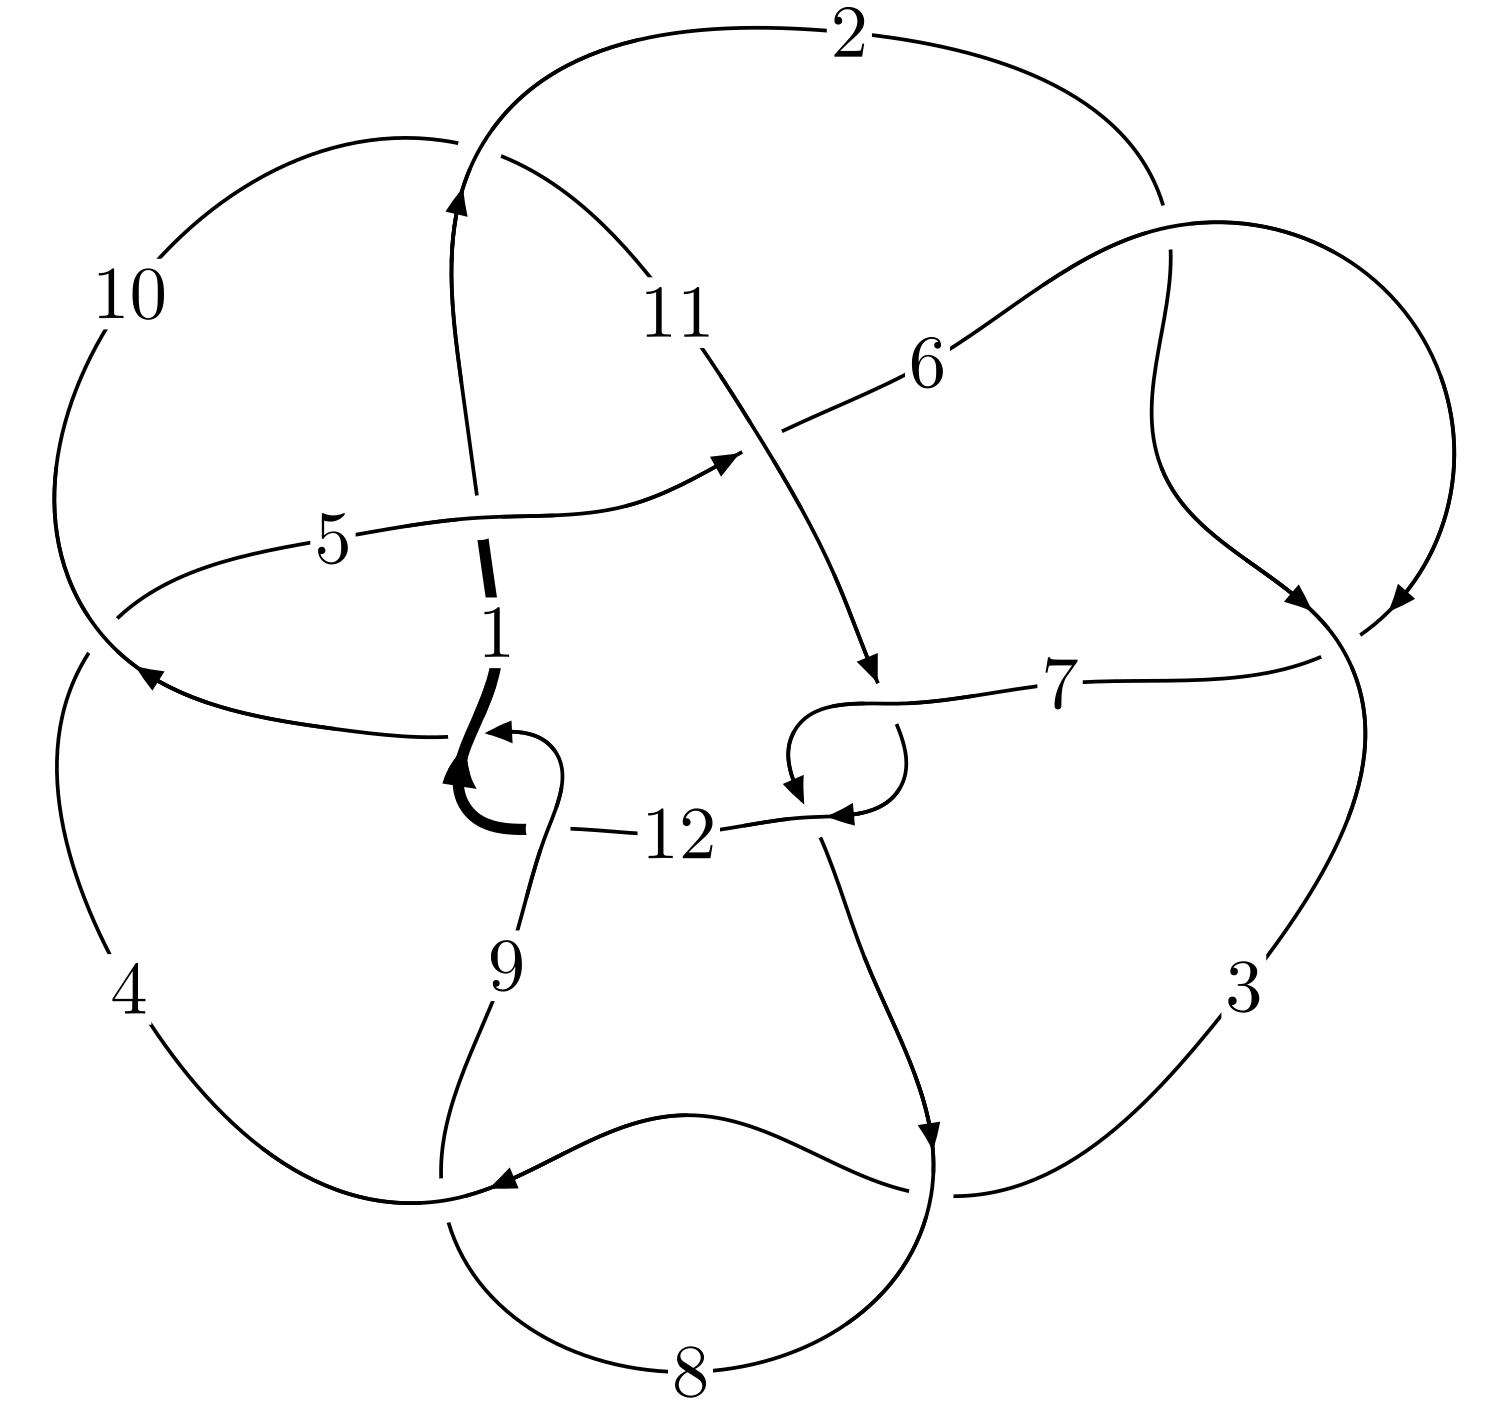
\includegraphics[width=112pt]{../../../GIT/diagram.site/Diagrams/png/2026_12a_1225.png}\\
\ \ \ A knot diagram\footnotemark}&
\allowdisplaybreaks
\textbf{Linearized knot diagam} \\
\cline{2-2}
 &
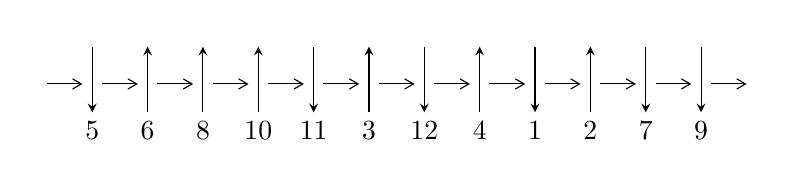
\begin{tikzpicture}[x=20pt, y=17pt]
	% nodes
	\node (C0) at (0, 0) {};
	\node (C1) at (1, 0) {};
	\node (C1U) at (1, +1) {};
	\node (C1D) at (1, -1) {5};

	\node (C2) at (2, 0) {};
	\node (C2U) at (2, +1) {};
	\node (C2D) at (2, -1) {6};

	\node (C3) at (3, 0) {};
	\node (C3U) at (3, +1) {};
	\node (C3D) at (3, -1) {8};

	\node (C4) at (4, 0) {};
	\node (C4U) at (4, +1) {};
	\node (C4D) at (4, -1) {10};

	\node (C5) at (5, 0) {};
	\node (C5U) at (5, +1) {};
	\node (C5D) at (5, -1) {11};

	\node (C6) at (6, 0) {};
	\node (C6U) at (6, +1) {};
	\node (C6D) at (6, -1) {3};

	\node (C7) at (7, 0) {};
	\node (C7U) at (7, +1) {};
	\node (C7D) at (7, -1) {12};

	\node (C8) at (8, 0) {};
	\node (C8U) at (8, +1) {};
	\node (C8D) at (8, -1) {4};

	\node (C9) at (9, 0) {};
	\node (C9U) at (9, +1) {};
	\node (C9D) at (9, -1) {1};

	\node (C10) at (10, 0) {};
	\node (C10U) at (10, +1) {};
	\node (C10D) at (10, -1) {2};

	\node (C11) at (11, 0) {};
	\node (C11U) at (11, +1) {};
	\node (C11D) at (11, -1) {7};

	\node (C12) at (12, 0) {};
	\node (C12U) at (12, +1) {};
	\node (C12D) at (12, -1) {9};
	\node (C13) at (13, 0) {};

	% arrows
	\draw[->,>={angle 60}]
	(C0) edge (C1) (C1) edge (C2) (C2) edge (C3) (C3) edge (C4) (C4) edge (C5) (C5) edge (C6) (C6) edge (C7) (C7) edge (C8) (C8) edge (C9) (C9) edge (C10) (C10) edge (C11) (C11) edge (C12) (C12) edge (C13) ;	\draw[->,>=stealth]
	(C1U) edge (C1D) (C2D) edge (C2U) (C3D) edge (C3U) (C4D) edge (C4U) (C5U) edge (C5D) (C6D) edge (C6U) (C7U) edge (C7D) (C8D) edge (C8U) (C9U) edge (C9D) (C10D) edge (C10U) (C11U) edge (C11D) (C12U) edge (C12D) ;
	\end{tikzpicture} \\
\hhline{~~} \\& 
\textbf{Solving Sequence} \\ \cline{2-2} 
 &
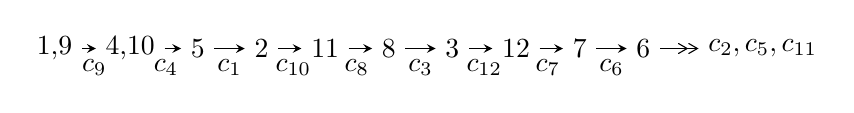
\begin{tikzpicture}[x=23pt, y=7pt]
	% node
	\node (A0) at (-1/8, 0) {1,9};
	\node (A1) at (17/16, 0) {4,10};
	\node (A2) at (17/8, 0) {5};
	\node (A3) at (25/8, 0) {2};
	\node (A4) at (33/8, 0) {11};
	\node (A5) at (41/8, 0) {8};
	\node (A6) at (49/8, 0) {3};
	\node (A7) at (57/8, 0) {12};
	\node (A8) at (65/8, 0) {7};
	\node (A9) at (73/8, 0) {6};
	\node (C1) at (1/2, -1) {$c_{9}$};
	\node (C2) at (13/8, -1) {$c_{4}$};
	\node (C3) at (21/8, -1) {$c_{1}$};
	\node (C4) at (29/8, -1) {$c_{10}$};
	\node (C5) at (37/8, -1) {$c_{8}$};
	\node (C6) at (45/8, -1) {$c_{3}$};
	\node (C7) at (53/8, -1) {$c_{12}$};
	\node (C8) at (61/8, -1) {$c_{7}$};
	\node (C9) at (69/8, -1) {$c_{6}$};
	\node (A10) at (11, 0) {$c_{2},c_{5},c_{11}$};

	% edge
	\draw[->,>=stealth]	
	(A0) edge (A1) (A1) edge (A2) (A2) edge (A3) (A3) edge (A4) (A4) edge (A5) (A5) edge (A6) (A6) edge (A7) (A7) edge (A8) (A8) edge (A9) ;
	\draw[->>,>={angle 60}]	
	(A9) edge (A10);
\end{tikzpicture} \\ 

\end{tabular} \\

\footnotetext{
The image of knot diagram is generated by the software ``\textbf{Draw programme}" developed by Andrew Bartholomew(\url{http://www.layer8.co.uk/maths/draw/index.htm\#Running-draw}), where we modified some parts for our purpose(\url{https://github.com/CATsTAILs/LinksPainter}).
}\phantom \\ \newline 
\centering \textbf{Ideals for irreducible components\footnotemark of $X_{\text{par}}$} 
 
\begin{align*}
I^u_{1}&=\langle 
7.20918\times10^{393} u^{111}+5.54525\times10^{394} u^{110}+\cdots+1.43090\times10^{397} b-3.89590\times10^{397},\\
\phantom{I^u_{1}}&\phantom{= \langle  }-1.74511\times10^{396} u^{111}-9.01477\times10^{395} u^{110}+\cdots+1.21484\times10^{400} a-9.13035\times10^{401},\\
\phantom{I^u_{1}}&\phantom{= \langle  }u^{112}+9 u^{111}+\cdots-90142 u-1132\rangle \\
I^u_{2}&=\langle 
-1343140997 u^{15}-3388091310 u^{14}+\cdots+6660374991 b+2076426241,\\
\phantom{I^u_{2}}&\phantom{= \langle  }265614140 u^{15}+2980660587 u^{14}+\cdots+6660374991 a+17049769085,\;u^{16}+5 u^{15}+\cdots-2 u-1\rangle \\
I^u_{3}&=\langle 
- a^3+b-4 a-1,\;a^4+a^3+4 a^2+4 a+1,\;u-1\rangle \\
I^u_{4}&=\langle 
b+1,\;a+1,\;u-1\rangle \\
I^u_{5}&=\langle 
b^5-2 b^4 a+b^3 a^2-3 b^3+4 b^2 a- a^2 b+b- a+1,\;u-1\rangle \\
\\
I^v_{1}&=\langle 
a,\;b^4+b^3-1,\;v-1\rangle \\
I^v_{2}&=\langle 
a,\;b-1,\;v-1\rangle \\
\end{align*}
\raggedright * 6 irreducible components of $\dim_{\mathbb{C}}=0$, with total 138 representations.\\
\raggedright * 1 irreducible components of $\dim_{\mathbb{C}}=1$ \\
\footnotetext{All coefficients of polynomials are rational numbers. But the coefficients are sometimes approximated in decimal forms when there is not enough margin.}
\newpage
\renewcommand{\arraystretch}{1}
\centering \section*{I. $I^u_{1}= \langle 7.21\times10^{393} u^{111}+5.55\times10^{394} u^{110}+\cdots+1.43\times10^{397} b-3.90\times10^{397},\;-1.75\times10^{396} u^{111}-9.01\times10^{395} u^{110}+\cdots+1.21\times10^{400} a-9.13\times10^{401},\;u^{112}+9 u^{111}+\cdots-90142 u-1132 \rangle$}
\flushleft \textbf{(i) Arc colorings}\\
\begin{tabular}{m{7pt} m{180pt} m{7pt} m{180pt} }
\flushright $a_{1}=$&$\begin{pmatrix}0\\u\end{pmatrix}$ \\
\flushright $a_{9}=$&$\begin{pmatrix}1\\0\end{pmatrix}$ \\
\flushright $a_{4}=$&$\begin{pmatrix}0.000143650 u^{111}+0.0000742056 u^{110}+\cdots+1183.64 u+75.1571\\-0.000503820 u^{111}-0.00387535 u^{110}+\cdots+132.583 u+2.72269\end{pmatrix}$ \\
\flushright $a_{10}=$&$\begin{pmatrix}1\\u^2\end{pmatrix}$ \\
\flushright $a_{5}=$&$\begin{pmatrix}-0.00163818 u^{111}-0.0140914 u^{110}+\cdots+1425.91 u+79.2593\\-0.00251920 u^{111}-0.0199229 u^{110}+\cdots+299.210 u+4.84051\end{pmatrix}$ \\
\flushright $a_{2}=$&$\begin{pmatrix}0.000256671 u^{111}+0.00161270 u^{110}+\cdots+1043.43 u+70.8299\\0.000551878 u^{111}+0.00433234 u^{110}+\cdots-57.9556 u+0.0777320\end{pmatrix}$ \\
\flushright $a_{11}=$&$\begin{pmatrix}0.000976338 u^{111}+0.00910943 u^{110}+\cdots-1193.78 u-61.3082\\-0.000854627 u^{111}-0.00682138 u^{110}+\cdots+94.3398 u+0.548443\end{pmatrix}$ \\
\flushright $a_{8}=$&$\begin{pmatrix}-0.000398981 u^{111}-0.00415660 u^{110}+\cdots+1073.25 u+68.4436\\0.000742676 u^{111}+0.00637617 u^{110}+\cdots-273.417 u-2.86495\end{pmatrix}$ \\
\flushright $a_{3}=$&$\begin{pmatrix}-0.00139747 u^{111}-0.0104758 u^{110}+\cdots-147.808 u+8.40896\\-0.00107238 u^{111}-0.00755752 u^{110}+\cdots-265.251 u-3.49103\end{pmatrix}$ \\
\flushright $a_{12}=$&$\begin{pmatrix}u\\u\end{pmatrix}$ \\
\flushright $a_{7}=$&$\begin{pmatrix}-0.000769701 u^{111}-0.00710499 u^{110}+\cdots+1097.78 u+68.7355\\0.000371956 u^{111}+0.00342777 u^{110}+\cdots-248.882 u-2.57307\end{pmatrix}$ \\
\flushright $a_{6}=$&$\begin{pmatrix}-0.000217324 u^{111}-0.00370821 u^{110}+\cdots+1742.49 u+88.6486\\0.000823128 u^{111}+0.00586181 u^{110}+\cdots+199.870 u+3.76570\end{pmatrix}$\\&\end{tabular}
\flushleft \textbf{(ii) Obstruction class $= -1$}\\~\\
\flushleft \textbf{(iii) Cusp Shapes $= 0.0107685 u^{111}+0.0968647 u^{110}+\cdots-5066.55 u-61.6765$}\\~\\
\newpage\renewcommand{\arraystretch}{1}
\flushleft \textbf{(iv) u-Polynomials at the component}\newline \\
\begin{tabular}{m{50pt}|m{274pt}}
Crossings & \hspace{64pt}u-Polynomials at each crossing \\
\hline $$\begin{aligned}c_{1}\end{aligned}$$&$\begin{aligned}
&16(16 u^{112}+8 u^{111}+\cdots-57723 u+15987)
\end{aligned}$\\
\hline $$\begin{aligned}c_{2},c_{6}\end{aligned}$$&$\begin{aligned}
&u^{112}+9 u^{111}+\cdots-90142 u-1132
\end{aligned}$\\
\hline $$\begin{aligned}c_{3},c_{8}\end{aligned}$$&$\begin{aligned}
&16(16 u^{112}-8 u^{111}+\cdots-75 u+75)
\end{aligned}$\\
\hline $$\begin{aligned}c_{4}\end{aligned}$$&$\begin{aligned}
&48(48 u^{112}-48 u^{111}+\cdots-1592 u-64)
\end{aligned}$\\
\hline $$\begin{aligned}c_{5}\end{aligned}$$&$\begin{aligned}
&48(48 u^{112}+48 u^{111}+\cdots+1592 u-64)
\end{aligned}$\\
\hline $$\begin{aligned}c_{7},c_{11}\end{aligned}$$&$\begin{aligned}
&16(16 u^{112}+8 u^{111}+\cdots+75 u+75)
\end{aligned}$\\
\hline $$\begin{aligned}c_{9},c_{12}\end{aligned}$$&$\begin{aligned}
&u^{112}-9 u^{111}+\cdots+90142 u-1132
\end{aligned}$\\
\hline $$\begin{aligned}c_{10}\end{aligned}$$&$\begin{aligned}
&16(16 u^{112}-8 u^{111}+\cdots+57723 u+15987)
\end{aligned}$\\
\hline
\end{tabular}\\~\\
\newpage\renewcommand{\arraystretch}{1}
\flushleft \textbf{(v) Riley Polynomials at the component}\newline \\
\begin{tabular}{m{50pt}|m{274pt}}
Crossings & \hspace{64pt}Riley Polynomials at each crossing \\
\hline $$\begin{aligned}c_{1},c_{10}\end{aligned}$$&$\begin{aligned}
&256(256 y^{112}-5152 y^{111}+\cdots-1.30933\times10^{10} y+2.55584\times10^{8})
\end{aligned}$\\
\hline $$\begin{aligned}c_{2},c_{6},c_{9}\\c_{12}\end{aligned}$$&$\begin{aligned}
&y^{112}-75 y^{111}+\cdots-5045677580 y+1281424
\end{aligned}$\\
\hline $$\begin{aligned}c_{3},c_{7},c_{8}\\c_{11}\end{aligned}$$&$\begin{aligned}
&256(256 y^{112}-16672 y^{111}+\cdots-439725 y+5625)
\end{aligned}$\\
\hline $$\begin{aligned}c_{4},c_{5}\end{aligned}$$&$\begin{aligned}
&2304(2304 y^{112}-11424 y^{111}+\cdots-1092032 y+4096)
\end{aligned}$\\
\hline
\end{tabular}\\~\\
\newpage\flushleft \textbf{(vi) Complex Volumes and Cusp Shapes}
$$\begin{array}{c|c|c}  
\text{Solutions to }I^u_{1}& \I (\text{vol} + \sqrt{-1}CS) & \text{Cusp shape}\\
 \hline 
\begin{aligned}
u &= -0.076594 + 0.998674 I \\
a &= \phantom{-}0.231384 + 0.192595 I \\
b &= -1.092480 + 0.313140 I\end{aligned}
 & \phantom{-}3.25749 - 3.93133 I & \phantom{-0.000000 } 0 \\ \hline\begin{aligned}
u &= -0.076594 - 0.998674 I \\
a &= \phantom{-}0.231384 - 0.192595 I \\
b &= -1.092480 - 0.313140 I\end{aligned}
 & \phantom{-}3.25749 + 3.93133 I & \phantom{-0.000000 } 0 \\ \hline\begin{aligned}
u &= \phantom{-}0.989446 + 0.111155 I \\
a &= -0.06785 - 2.70572 I \\
b &= \phantom{-}0.26976 - 1.69355 I\end{aligned}
 & -0.179102 + 1.361240 I & \phantom{-0.000000 } 0 \\ \hline\begin{aligned}
u &= \phantom{-}0.989446 - 0.111155 I \\
a &= -0.06785 + 2.70572 I \\
b &= \phantom{-}0.26976 + 1.69355 I\end{aligned}
 & -0.179102 - 1.361240 I & \phantom{-0.000000 } 0 \\ \hline\begin{aligned}
u &= \phantom{-}1.03475\phantom{ +0.000000I} \\
a &= -0.678980\phantom{ +0.000000I} \\
b &= -0.837668\phantom{ +0.000000I}\end{aligned}
 & -1.64218\phantom{ +0.000000I} & \phantom{-0.000000 } 0 \\ \hline\begin{aligned}
u &= -0.928213 + 0.201967 I \\
a &= \phantom{-}0.799418 - 0.944826 I \\
b &= \phantom{-}1.170730 - 0.590714 I\end{aligned}
 & \phantom{-}0.866138 + 0.769169 I & \phantom{-0.000000 } 0 \\ \hline\begin{aligned}
u &= -0.928213 - 0.201967 I \\
a &= \phantom{-}0.799418 + 0.944826 I \\
b &= \phantom{-}1.170730 + 0.590714 I\end{aligned}
 & \phantom{-}0.866138 - 0.769169 I & \phantom{-0.000000 } 0 \\ \hline\begin{aligned}
u &= \phantom{-}0.012899 + 1.051640 I \\
a &= -0.263753 - 0.403519 I \\
b &= \phantom{-}1.333720 - 0.114397 I\end{aligned}
 & \phantom{-}8.41416 - 6.54605 I & \phantom{-0.000000 } 0 \\ \hline\begin{aligned}
u &= \phantom{-}0.012899 - 1.051640 I \\
a &= -0.263753 + 0.403519 I \\
b &= \phantom{-}1.333720 + 0.114397 I\end{aligned}
 & \phantom{-}8.41416 + 6.54605 I & \phantom{-0.000000 } 0 \\ \hline\begin{aligned}
u &= -0.033862 + 0.928112 I \\
a &= -0.140232 + 0.039291 I \\
b &= \phantom{-}1.281230 - 0.478890 I\end{aligned}
 & \phantom{-}5.94038 - 4.98070 I & \phantom{-0.000000 } 0\\
 \hline 
 \end{array}$$\newpage$$\begin{array}{c|c|c}  
\text{Solutions to }I^u_{1}& \I (\text{vol} + \sqrt{-1}CS) & \text{Cusp shape}\\
 \hline 
\begin{aligned}
u &= -0.033862 - 0.928112 I \\
a &= -0.140232 - 0.039291 I \\
b &= \phantom{-}1.281230 + 0.478890 I\end{aligned}
 & \phantom{-}5.94038 + 4.98070 I & \phantom{-0.000000 } 0 \\ \hline\begin{aligned}
u &= -0.842253 + 0.386957 I \\
a &= \phantom{-}0.47697 - 1.50961 I \\
b &= \phantom{-}0.239501 + 0.060068 I\end{aligned}
 & \phantom{-}0.62344 + 9.53417 I & \phantom{-0.000000 } 0 \\ \hline\begin{aligned}
u &= -0.842253 - 0.386957 I \\
a &= \phantom{-}0.47697 + 1.50961 I \\
b &= \phantom{-}0.239501 - 0.060068 I\end{aligned}
 & \phantom{-}0.62344 - 9.53417 I & \phantom{-0.000000 } 0 \\ \hline\begin{aligned}
u &= -1.042910 + 0.349738 I \\
a &= -0.383966 + 1.323600 I \\
b &= -0.281312 + 0.605442 I\end{aligned}
 & -2.67525 + 4.55404 I & \phantom{-0.000000 } 0 \\ \hline\begin{aligned}
u &= -1.042910 - 0.349738 I \\
a &= -0.383966 - 1.323600 I \\
b &= -0.281312 - 0.605442 I\end{aligned}
 & -2.67525 - 4.55404 I & \phantom{-0.000000 } 0 \\ \hline\begin{aligned}
u &= -0.808934 + 0.384457 I \\
a &= \phantom{-}0.15671 + 1.60302 I \\
b &= \phantom{-}0.780624 + 0.552924 I\end{aligned}
 & \phantom{-}1.13362 + 2.05532 I & \phantom{-0.000000 } 0 \\ \hline\begin{aligned}
u &= -0.808934 - 0.384457 I \\
a &= \phantom{-}0.15671 - 1.60302 I \\
b &= \phantom{-}0.780624 - 0.552924 I\end{aligned}
 & \phantom{-}1.13362 - 2.05532 I & \phantom{-0.000000 } 0 \\ \hline\begin{aligned}
u &= \phantom{-}1.048220 + 0.374459 I \\
a &= -0.869926 - 0.251124 I \\
b &= -0.291121 - 0.253138 I\end{aligned}
 & -0.866138 + 0.769169 I & \phantom{-0.000000 } 0 \\ \hline\begin{aligned}
u &= \phantom{-}1.048220 - 0.374459 I \\
a &= -0.869926 + 0.251124 I \\
b &= -0.291121 + 0.253138 I\end{aligned}
 & -0.866138 - 0.769169 I & \phantom{-0.000000 } 0 \\ \hline\begin{aligned}
u &= \phantom{-}1.072650 + 0.309982 I \\
a &= \phantom{-}0.08998 + 2.27104 I \\
b &= -0.829938 + 0.206066 I\end{aligned}
 & \phantom{-}0.179102 - 1.361240 I & \phantom{-0.000000 } 0\\
 \hline 
 \end{array}$$\newpage$$\begin{array}{c|c|c}  
\text{Solutions to }I^u_{1}& \I (\text{vol} + \sqrt{-1}CS) & \text{Cusp shape}\\
 \hline 
\begin{aligned}
u &= \phantom{-}1.072650 - 0.309982 I \\
a &= \phantom{-}0.08998 - 2.27104 I \\
b &= -0.829938 - 0.206066 I\end{aligned}
 & \phantom{-}0.179102 + 1.361240 I & \phantom{-0.000000 } 0 \\ \hline\begin{aligned}
u &= \phantom{-}0.771213 + 0.378608 I \\
a &= -0.583767 + 0.056030 I \\
b &= -0.859928 - 0.546705 I\end{aligned}
 & -2.02176 + 0.22367 I & \phantom{-0.000000 } 0 \\ \hline\begin{aligned}
u &= \phantom{-}0.771213 - 0.378608 I \\
a &= -0.583767 - 0.056030 I \\
b &= -0.859928 + 0.546705 I\end{aligned}
 & -2.02176 - 0.22367 I & \phantom{-0.000000 } 0 \\ \hline\begin{aligned}
u &= -0.229968 + 0.823116 I \\
a &= \phantom{-}0.053000 - 0.318049 I \\
b &= -1.397590 - 0.020177 I\end{aligned}
 & \phantom{-}9.29392 - 0.40910 I & \phantom{-0.000000 } 0 \\ \hline\begin{aligned}
u &= -0.229968 - 0.823116 I \\
a &= \phantom{-}0.053000 + 0.318049 I \\
b &= -1.397590 + 0.020177 I\end{aligned}
 & \phantom{-}9.29392 + 0.40910 I & \phantom{-0.000000 } 0 \\ \hline\begin{aligned}
u &= \phantom{-}0.473129 + 1.051400 I \\
a &= \phantom{-}0.199711 - 0.300992 I \\
b &= \phantom{-}1.198560 + 0.396998 I\end{aligned}
 & \phantom{-}5.00780 + 5.56131 I & \phantom{-0.000000 } 0 \\ \hline\begin{aligned}
u &= \phantom{-}0.473129 - 1.051400 I \\
a &= \phantom{-}0.199711 + 0.300992 I \\
b &= \phantom{-}1.198560 - 0.396998 I\end{aligned}
 & \phantom{-}5.00780 - 5.56131 I & \phantom{-0.000000 } 0 \\ \hline\begin{aligned}
u &= -1.145040 + 0.158811 I \\
a &= \phantom{-}0.12713 - 1.42460 I \\
b &= -1.228560 - 0.577397 I\end{aligned}
 & -5.94038 + 4.98070 I & \phantom{-0.000000 } 0 \\ \hline\begin{aligned}
u &= -1.145040 - 0.158811 I \\
a &= \phantom{-}0.12713 + 1.42460 I \\
b &= -1.228560 + 0.577397 I\end{aligned}
 & -5.94038 - 4.98070 I & \phantom{-0.000000 } 0 \\ \hline\begin{aligned}
u &= -1.155800 + 0.143605 I \\
a &= -0.04341 + 1.85196 I \\
b &= \phantom{-}1.184810 + 0.664213 I\end{aligned}
 & -1.99720 + 9.98062 I & \phantom{-0.000000 } 0\\
 \hline 
 \end{array}$$\newpage$$\begin{array}{c|c|c}  
\text{Solutions to }I^u_{1}& \I (\text{vol} + \sqrt{-1}CS) & \text{Cusp shape}\\
 \hline 
\begin{aligned}
u &= -1.155800 - 0.143605 I \\
a &= -0.04341 - 1.85196 I \\
b &= \phantom{-}1.184810 - 0.664213 I\end{aligned}
 & -1.99720 - 9.98062 I & \phantom{-0.000000 } 0 \\ \hline\begin{aligned}
u &= \phantom{-}0.497490 + 0.652853 I \\
a &= \phantom{-}0.568345 + 0.080588 I \\
b &= -0.127788 - 0.410063 I\end{aligned}
 & -1.13362 - 2.05532 I & \phantom{-0.000000 } 0 \\ \hline\begin{aligned}
u &= \phantom{-}0.497490 - 0.652853 I \\
a &= \phantom{-}0.568345 - 0.080588 I \\
b &= -0.127788 + 0.410063 I\end{aligned}
 & -1.13362 + 2.05532 I & \phantom{-0.000000 } 0 \\ \hline\begin{aligned}
u &= \phantom{-}0.941206 + 0.736070 I \\
a &= \phantom{-}0.381307 + 1.186970 I \\
b &= -1.056170 + 0.634618 I\end{aligned}
 & -1.25247 - 5.17059 I & \phantom{-0.000000 } 0 \\ \hline\begin{aligned}
u &= \phantom{-}0.941206 - 0.736070 I \\
a &= \phantom{-}0.381307 - 1.186970 I \\
b &= -1.056170 - 0.634618 I\end{aligned}
 & -1.25247 + 5.17059 I & \phantom{-0.000000 } 0 \\ \hline\begin{aligned}
u &= -1.084390 + 0.505444 I \\
a &= -0.510177 - 1.293310 I \\
b &= -1.270000 - 0.369732 I\end{aligned}
 & \phantom{-}6.78188 + 5.23022 I & \phantom{-0.000000 } 0 \\ \hline\begin{aligned}
u &= -1.084390 - 0.505444 I \\
a &= -0.510177 + 1.293310 I \\
b &= -1.270000 + 0.369732 I\end{aligned}
 & \phantom{-}6.78188 - 5.23022 I & \phantom{-0.000000 } 0 \\ \hline\begin{aligned}
u &= -1.190100 + 0.153253 I \\
a &= \phantom{-}0.178297 + 0.610262 I \\
b &= \phantom{-}1.38897 + 0.33779 I\end{aligned}
 & -1.46756 + 0.33645 I & \phantom{-0.000000 } 0 \\ \hline\begin{aligned}
u &= -1.190100 - 0.153253 I \\
a &= \phantom{-}0.178297 - 0.610262 I \\
b &= \phantom{-}1.38897 - 0.33779 I\end{aligned}
 & -1.46756 - 0.33645 I & \phantom{-0.000000 } 0 \\ \hline\begin{aligned}
u &= -0.122047 + 0.779373 I \\
a &= -0.114156 + 0.418854 I \\
b &= -0.527172 + 0.483285 I\end{aligned}
 & \phantom{-}2.67525 - 4.55404 I & \phantom{-0.000000 } 0\\
 \hline 
 \end{array}$$\newpage$$\begin{array}{c|c|c}  
\text{Solutions to }I^u_{1}& \I (\text{vol} + \sqrt{-1}CS) & \text{Cusp shape}\\
 \hline 
\begin{aligned}
u &= -0.122047 - 0.779373 I \\
a &= -0.114156 - 0.418854 I \\
b &= -0.527172 - 0.483285 I\end{aligned}
 & \phantom{-}2.67525 + 4.55404 I & \phantom{-0.000000 } 0 \\ \hline\begin{aligned}
u &= \phantom{-}1.069800 + 0.576020 I \\
a &= \phantom{-}0.14524 - 1.44287 I \\
b &= \phantom{-}1.36776 - 0.79349 I\end{aligned}
 & \phantom{-}3.04906 - 11.28170 I & \phantom{-0.000000 } 0 \\ \hline\begin{aligned}
u &= \phantom{-}1.069800 - 0.576020 I \\
a &= \phantom{-}0.14524 + 1.44287 I \\
b &= \phantom{-}1.36776 + 0.79349 I\end{aligned}
 & \phantom{-}3.04906 + 11.28170 I & \phantom{-0.000000 } 0 \\ \hline\begin{aligned}
u &= -0.023540 + 1.254960 I \\
a &= \phantom{-}0.449621 - 0.002989 I \\
b &= -1.059750 + 0.329925 I\end{aligned}
 & \phantom{-}1.25247 - 5.17059 I & \phantom{-0.000000 } 0 \\ \hline\begin{aligned}
u &= -0.023540 - 1.254960 I \\
a &= \phantom{-}0.449621 + 0.002989 I \\
b &= -1.059750 - 0.329925 I\end{aligned}
 & \phantom{-}1.25247 + 5.17059 I & \phantom{-0.000000 } 0 \\ \hline\begin{aligned}
u &= -0.150701 + 1.283400 I \\
a &= \phantom{-}0.141625 - 0.115575 I \\
b &= -1.253310 - 0.414045 I\end{aligned}
 & \phantom{-}4.91352 + 13.09700 I & \phantom{-0.000000 } 0 \\ \hline\begin{aligned}
u &= -0.150701 - 1.283400 I \\
a &= \phantom{-}0.141625 + 0.115575 I \\
b &= -1.253310 + 0.414045 I\end{aligned}
 & \phantom{-}4.91352 - 13.09700 I & \phantom{-0.000000 } 0 \\ \hline\begin{aligned}
u &= \phantom{-}1.267280 + 0.341348 I \\
a &= \phantom{-}0.60742 - 1.44572 I \\
b &= \phantom{-}0.895900 - 0.360926 I\end{aligned}
 & -1.28303 - 3.24310 I & \phantom{-0.000000 } 0 \\ \hline\begin{aligned}
u &= \phantom{-}1.267280 - 0.341348 I \\
a &= \phantom{-}0.60742 + 1.44572 I \\
b &= \phantom{-}0.895900 + 0.360926 I\end{aligned}
 & -1.28303 + 3.24310 I & \phantom{-0.000000 } 0 \\ \hline\begin{aligned}
u &= \phantom{-}1.303300 + 0.294422 I \\
a &= -0.11471 - 1.55010 I \\
b &= -0.07325 - 1.51517 I\end{aligned}
 & -4.13502 - 12.09070 I & \phantom{-0.000000 } 0\\
 \hline 
 \end{array}$$\newpage$$\begin{array}{c|c|c}  
\text{Solutions to }I^u_{1}& \I (\text{vol} + \sqrt{-1}CS) & \text{Cusp shape}\\
 \hline 
\begin{aligned}
u &= \phantom{-}1.303300 - 0.294422 I \\
a &= -0.11471 + 1.55010 I \\
b &= -0.07325 + 1.51517 I\end{aligned}
 & -4.13502 + 12.09070 I & \phantom{-0.000000 } 0 \\ \hline\begin{aligned}
u &= \phantom{-}1.194340 + 0.660141 I \\
a &= \phantom{-}0.210808 + 0.809537 I \\
b &= -0.763792 + 0.253689 I\end{aligned}
 & -1.72504 - 2.62810 I & \phantom{-0.000000 } 0 \\ \hline\begin{aligned}
u &= \phantom{-}1.194340 - 0.660141 I \\
a &= \phantom{-}0.210808 - 0.809537 I \\
b &= -0.763792 - 0.253689 I\end{aligned}
 & -1.72504 + 2.62810 I & \phantom{-0.000000 } 0 \\ \hline\begin{aligned}
u &= -1.263900 + 0.516886 I \\
a &= -0.03228 - 1.44001 I \\
b &= -0.829618 - 0.750072 I\end{aligned}
 & -0.62344 + 9.53417 I & \phantom{-0.000000 } 0 \\ \hline\begin{aligned}
u &= -1.263900 - 0.516886 I \\
a &= -0.03228 + 1.44001 I \\
b &= -0.829618 + 0.750072 I\end{aligned}
 & -0.62344 - 9.53417 I & \phantom{-0.000000 } 0 \\ \hline\begin{aligned}
u &= \phantom{-}1.334180 + 0.314698 I \\
a &= \phantom{-}0.081026 + 1.235020 I \\
b &= \phantom{-}0.198328 + 1.226370 I\end{aligned}
 & -8.41416 - 6.54605 I & \phantom{-0.000000 } 0 \\ \hline\begin{aligned}
u &= \phantom{-}1.334180 - 0.314698 I \\
a &= \phantom{-}0.081026 - 1.235020 I \\
b &= \phantom{-}0.198328 - 1.226370 I\end{aligned}
 & -8.41416 + 6.54605 I & \phantom{-0.000000 } 0 \\ \hline\begin{aligned}
u &= \phantom{-}0.328035 + 0.535610 I \\
a &= -1.188290 + 0.333926 I \\
b &= \phantom{-}1.095590 - 0.102708 I\end{aligned}
 & \phantom{-}2.02176 - 0.22367 I & \phantom{-}4.79873 + 0.86633 I \\ \hline\begin{aligned}
u &= \phantom{-}0.328035 - 0.535610 I \\
a &= -1.188290 - 0.333926 I \\
b &= \phantom{-}1.095590 + 0.102708 I\end{aligned}
 & \phantom{-}2.02176 + 0.22367 I & \phantom{-}4.79873 - 0.86633 I \\ \hline\begin{aligned}
u &= -1.352620 + 0.255718 I \\
a &= -0.196044 + 1.169210 I \\
b &= -0.118555 + 1.122180 I\end{aligned}
 & -6.78188 + 5.23022 I & \phantom{-0.000000 } 0\\
 \hline 
 \end{array}$$\newpage$$\begin{array}{c|c|c}  
\text{Solutions to }I^u_{1}& \I (\text{vol} + \sqrt{-1}CS) & \text{Cusp shape}\\
 \hline 
\begin{aligned}
u &= -1.352620 - 0.255718 I \\
a &= -0.196044 - 1.169210 I \\
b &= -0.118555 - 1.122180 I\end{aligned}
 & -6.78188 - 5.23022 I & \phantom{-0.000000 } 0 \\ \hline\begin{aligned}
u &= -1.298990 + 0.466389 I \\
a &= \phantom{-}0.37182 + 1.60795 I \\
b &= \phantom{-}1.35303 + 0.86227 I\end{aligned}
 & \phantom{-}1.99720 + 9.98062 I & \phantom{-0.000000 } 0 \\ \hline\begin{aligned}
u &= -1.298990 - 0.466389 I \\
a &= \phantom{-}0.37182 - 1.60795 I \\
b &= \phantom{-}1.35303 - 0.86227 I\end{aligned}
 & \phantom{-}1.99720 - 9.98062 I & \phantom{-0.000000 } 0 \\ \hline\begin{aligned}
u &= -1.385620 + 0.052575 I \\
a &= \phantom{-}0.73344 + 1.28348 I \\
b &= \phantom{-}0.485042 + 1.057350 I\end{aligned}
 & -4.28714 - 3.78788 I & \phantom{-0.000000 } 0 \\ \hline\begin{aligned}
u &= -1.385620 - 0.052575 I \\
a &= \phantom{-}0.73344 - 1.28348 I \\
b &= \phantom{-}0.485042 - 1.057350 I\end{aligned}
 & -4.28714 + 3.78788 I & \phantom{-0.000000 } 0 \\ \hline\begin{aligned}
u &= -1.310370 + 0.516292 I \\
a &= -0.21364 - 1.43619 I \\
b &= -1.092980 - 0.635421 I\end{aligned}
 & -0.61110 + 9.33643 I & \phantom{-0.000000 } 0 \\ \hline\begin{aligned}
u &= -1.310370 - 0.516292 I \\
a &= -0.21364 + 1.43619 I \\
b &= -1.092980 + 0.635421 I\end{aligned}
 & -0.61110 - 9.33643 I & \phantom{-0.000000 } 0 \\ \hline\begin{aligned}
u &= \phantom{-}1.37817 + 0.36293 I \\
a &= -0.84923 + 1.26582 I \\
b &= -1.240840 + 0.469570 I\end{aligned}
 & \phantom{-}4.28714 - 3.78788 I & \phantom{-0.000000 } 0 \\ \hline\begin{aligned}
u &= \phantom{-}1.37817 - 0.36293 I \\
a &= -0.84923 - 1.26582 I \\
b &= -1.240840 - 0.469570 I\end{aligned}
 & \phantom{-}4.28714 + 3.78788 I & \phantom{-0.000000 } 0 \\ \hline\begin{aligned}
u &= -1.43190 + 0.15558 I \\
a &= -0.203034 - 0.989310 I \\
b &= -0.080939 - 0.939558 I\end{aligned}
 & -9.29392 + 0.40910 I & \phantom{-0.000000 } 0\\
 \hline 
 \end{array}$$\newpage$$\begin{array}{c|c|c}  
\text{Solutions to }I^u_{1}& \I (\text{vol} + \sqrt{-1}CS) & \text{Cusp shape}\\
 \hline 
\begin{aligned}
u &= -1.43190 - 0.15558 I \\
a &= -0.203034 + 0.989310 I \\
b &= -0.080939 + 0.939558 I\end{aligned}
 & -9.29392 - 0.40910 I & \phantom{-0.000000 } 0 \\ \hline\begin{aligned}
u &= \phantom{-}1.41028 + 0.32457 I \\
a &= \phantom{-}0.757729 - 0.381296 I \\
b &= \phantom{-}0.925369 + 0.082252 I\end{aligned}
 & \phantom{-}1.46756 + 0.33645 I & \phantom{-0.000000 } 0 \\ \hline\begin{aligned}
u &= \phantom{-}1.41028 - 0.32457 I \\
a &= \phantom{-}0.757729 + 0.381296 I \\
b &= \phantom{-}0.925369 - 0.082252 I\end{aligned}
 & \phantom{-}1.46756 - 0.33645 I & \phantom{-0.000000 } 0 \\ \hline\begin{aligned}
u &= -0.365915 + 0.412674 I \\
a &= -0.14055 + 2.53139 I \\
b &= \phantom{-}0.253914 - 0.136115 I\end{aligned}
 & \phantom{-}1.72504 + 2.62810 I & \phantom{-}9.23789 - 9.47130 I \\ \hline\begin{aligned}
u &= -0.365915 - 0.412674 I \\
a &= -0.14055 - 2.53139 I \\
b &= \phantom{-}0.253914 + 0.136115 I\end{aligned}
 & \phantom{-}1.72504 - 2.62810 I & \phantom{-}9.23789 + 9.47130 I \\ \hline\begin{aligned}
u &= -1.35458 + 0.51347 I \\
a &= \phantom{-}0.44715 + 1.41303 I \\
b &= \phantom{-}1.219040 + 0.364948 I\end{aligned}
 & \phantom{-}4.13502 + 12.09070 I & \phantom{-0.000000 } 0 \\ \hline\begin{aligned}
u &= -1.35458 - 0.51347 I \\
a &= \phantom{-}0.44715 - 1.41303 I \\
b &= \phantom{-}1.219040 - 0.364948 I\end{aligned}
 & \phantom{-}4.13502 - 12.09070 I & \phantom{-0.000000 } 0 \\ \hline\begin{aligned}
u &= -1.09380 + 0.98488 I \\
a &= -0.223478 + 0.718541 I \\
b &= \phantom{-}0.664565 - 0.021277 I\end{aligned}
 & -2.08701 + 3.74779 I & \phantom{-0.000000 } 0 \\ \hline\begin{aligned}
u &= -1.09380 - 0.98488 I \\
a &= -0.223478 - 0.718541 I \\
b &= \phantom{-}0.664565 + 0.021277 I\end{aligned}
 & -2.08701 - 3.74779 I & \phantom{-0.000000 } 0 \\ \hline\begin{aligned}
u &= -0.42099 + 1.41567 I \\
a &= \phantom{-}0.249353 + 0.126700 I \\
b &= -0.968329 - 0.139295 I\end{aligned}
 & \phantom{-}2.08701 - 3.74779 I & \phantom{-0.000000 } 0\\
 \hline 
 \end{array}$$\newpage$$\begin{array}{c|c|c}  
\text{Solutions to }I^u_{1}& \I (\text{vol} + \sqrt{-1}CS) & \text{Cusp shape}\\
 \hline 
\begin{aligned}
u &= -0.42099 - 1.41567 I \\
a &= \phantom{-}0.249353 - 0.126700 I \\
b &= -0.968329 + 0.139295 I\end{aligned}
 & \phantom{-}2.08701 + 3.74779 I & \phantom{-0.000000 } 0 \\ \hline\begin{aligned}
u &= -1.37062 + 0.55200 I \\
a &= -0.063610 - 1.279610 I \\
b &= -1.31742 - 0.59639 I\end{aligned}
 & -3.04906 + 11.28170 I & \phantom{-0.000000 } 0 \\ \hline\begin{aligned}
u &= -1.37062 - 0.55200 I \\
a &= -0.063610 + 1.279610 I \\
b &= -1.31742 + 0.59639 I\end{aligned}
 & -3.04906 - 11.28170 I & \phantom{-0.000000 } 0 \\ \hline\begin{aligned}
u &= \phantom{-}0.349248 + 0.305350 I \\
a &= \phantom{-}0.768121 + 0.016112 I \\
b &= \phantom{-}0.739773 + 0.980194 I\end{aligned}
 & \phantom{-}1.28303 - 3.24310 I & \phantom{-}3.29814 + 8.40281 I \\ \hline\begin{aligned}
u &= \phantom{-}0.349248 - 0.305350 I \\
a &= \phantom{-}0.768121 - 0.016112 I \\
b &= \phantom{-}0.739773 - 0.980194 I\end{aligned}
 & \phantom{-}1.28303 + 3.24310 I & \phantom{-}3.29814 - 8.40281 I \\ \hline\begin{aligned}
u &= \phantom{-}1.48918 + 0.38329 I \\
a &= \phantom{-}0.061872 - 0.544415 I \\
b &= -0.413632 - 0.594403 I\end{aligned}
 & -4.00511 - 0.72764 I & \phantom{-0.000000 } 0 \\ \hline\begin{aligned}
u &= \phantom{-}1.48918 - 0.38329 I \\
a &= \phantom{-}0.061872 + 0.544415 I \\
b &= -0.413632 + 0.594403 I\end{aligned}
 & -4.00511 + 0.72764 I & \phantom{-0.000000 } 0 \\ \hline\begin{aligned}
u &= -0.046450 + 0.453850 I \\
a &= \phantom{-}0.824444 - 0.751338 I \\
b &= \phantom{-}0.115446 - 0.445470 I\end{aligned}
 & \phantom{-0.000000 } -1.27033 I & \phantom{-0.000000 -}0. + 4.50236 I \\ \hline\begin{aligned}
u &= -0.046450 - 0.453850 I \\
a &= \phantom{-}0.824444 + 0.751338 I \\
b &= \phantom{-}0.115446 + 0.445470 I\end{aligned}
 & \phantom{-0.000000 -}1.27033 I & \phantom{-0.000000 } 0. - 4.50236 I \\ \hline\begin{aligned}
u &= \phantom{-}1.44276 + 0.57759 I \\
a &= -0.298746 + 1.328770 I \\
b &= -1.41290 + 0.70903 I\end{aligned}
 & \phantom{-0.000000 } -19.5476 I & \phantom{-0.000000 } 0\\
 \hline 
 \end{array}$$\newpage$$\begin{array}{c|c|c}  
\text{Solutions to }I^u_{1}& \I (\text{vol} + \sqrt{-1}CS) & \text{Cusp shape}\\
 \hline 
\begin{aligned}
u &= \phantom{-}1.44276 - 0.57759 I \\
a &= -0.298746 - 1.328770 I \\
b &= -1.41290 - 0.70903 I\end{aligned}
 & \phantom{-0.000000 -}19.5476 I & \phantom{-0.000000 } 0 \\ \hline\begin{aligned}
u &= \phantom{-}1.45797 + 0.63871 I \\
a &= \phantom{-}0.181999 - 1.166490 I \\
b &= \phantom{-}1.31547 - 0.65832 I\end{aligned}
 & -4.91352 - 13.09700 I & \phantom{-0.000000 } 0 \\ \hline\begin{aligned}
u &= \phantom{-}1.45797 - 0.63871 I \\
a &= \phantom{-}0.181999 + 1.166490 I \\
b &= \phantom{-}1.31547 + 0.65832 I\end{aligned}
 & -4.91352 + 13.09700 I & \phantom{-0.000000 } 0 \\ \hline\begin{aligned}
u &= -0.309714 + 0.264226 I \\
a &= \phantom{-}2.48579 - 1.07022 I \\
b &= \phantom{-}0.452397 + 0.657328 I\end{aligned}
 & \phantom{-}0.61110 + 9.33643 I & -0.22464 - 7.70849 I \\ \hline\begin{aligned}
u &= -0.309714 - 0.264226 I \\
a &= \phantom{-}2.48579 + 1.07022 I \\
b &= \phantom{-}0.452397 - 0.657328 I\end{aligned}
 & \phantom{-}0.61110 - 9.33643 I & -0.22464 + 7.70849 I \\ \hline\begin{aligned}
u &= -1.50628 + 0.58589 I \\
a &= \phantom{-}0.154270 + 0.911151 I \\
b &= \phantom{-}1.33432 + 0.49940 I\end{aligned}
 & -5.00780 + 5.56131 I & \phantom{-0.000000 } 0 \\ \hline\begin{aligned}
u &= -1.50628 - 0.58589 I \\
a &= \phantom{-}0.154270 - 0.911151 I \\
b &= \phantom{-}1.33432 - 0.49940 I\end{aligned}
 & -5.00780 - 5.56131 I & \phantom{-0.000000 } 0 \\ \hline\begin{aligned}
u &= -0.19099 + 1.61396 I \\
a &= -0.1113280 + 0.0382015 I \\
b &= \phantom{-}1.103820 + 0.299690 I\end{aligned}
 & \phantom{-0.000000 -}5.74733 I & \phantom{-0.000000 } 0 \\ \hline\begin{aligned}
u &= -0.19099 - 1.61396 I \\
a &= -0.1113280 - 0.0382015 I \\
b &= \phantom{-}1.103820 - 0.299690 I\end{aligned}
 & \phantom{-0.000000 } -5.74733 I & \phantom{-0.000000 } 0 \\ \hline\begin{aligned}
u &= \phantom{-}1.35740 + 0.90914 I \\
a &= \phantom{-}0.128278 + 0.818090 I \\
b &= -1.105390 + 0.487764 I\end{aligned}
 & -1.96231 - 5.07117 I & \phantom{-0.000000 } 0\\
 \hline 
 \end{array}$$\newpage$$\begin{array}{c|c|c}  
\text{Solutions to }I^u_{1}& \I (\text{vol} + \sqrt{-1}CS) & \text{Cusp shape}\\
 \hline 
\begin{aligned}
u &= \phantom{-}1.35740 - 0.90914 I \\
a &= \phantom{-}0.128278 - 0.818090 I \\
b &= -1.105390 - 0.487764 I\end{aligned}
 & -1.96231 + 5.07117 I & \phantom{-0.000000 } 0 \\ \hline\begin{aligned}
u &= \phantom{-}1.52288 + 0.59787 I \\
a &= \phantom{-}0.375475 - 0.409323 I \\
b &= \phantom{-}1.356790 - 0.132401 I\end{aligned}
 & \phantom{-}4.00511 + 0.72764 I & \phantom{-0.000000 } 0 \\ \hline\begin{aligned}
u &= \phantom{-}1.52288 - 0.59787 I \\
a &= \phantom{-}0.375475 + 0.409323 I \\
b &= \phantom{-}1.356790 + 0.132401 I\end{aligned}
 & \phantom{-}4.00511 - 0.72764 I & \phantom{-0.000000 } 0 \\ \hline\begin{aligned}
u &= -1.63935\phantom{ +0.000000I} \\
a &= -0.478929\phantom{ +0.000000I} \\
b &= -0.242092\phantom{ +0.000000I}\end{aligned}
 & -10.3706\phantom{ +0.000000I} & \phantom{-0.000000 } 0 \\ \hline\begin{aligned}
u &= -1.07002 + 1.27061 I \\
a &= \phantom{-}0.030202 - 0.435703 I \\
b &= -0.927485 + 0.155970 I\end{aligned}
 & \phantom{-}1.96231 - 5.07117 I & \phantom{-0.000000 } 0 \\ \hline\begin{aligned}
u &= -1.07002 - 1.27061 I \\
a &= \phantom{-}0.030202 + 0.435703 I \\
b &= -0.927485 - 0.155970 I\end{aligned}
 & \phantom{-}1.96231 + 5.07117 I & \phantom{-0.000000 } 0 \\ \hline\begin{aligned}
u &= -0.290654 + 0.105986 I \\
a &= -3.69871 + 1.83262 I \\
b &= -0.514232 - 0.449850 I\end{aligned}
 & -3.25749 + 3.93133 I & -6.45843 - 5.67906 I \\ \hline\begin{aligned}
u &= -0.290654 - 0.105986 I \\
a &= -3.69871 - 1.83262 I \\
b &= -0.514232 + 0.449850 I\end{aligned}
 & -3.25749 - 3.93133 I & -6.45843 + 5.67906 I \\ \hline\begin{aligned}
u &= -0.187718\phantom{ +0.000000I} \\
a &= -1.90046\phantom{ +0.000000I} \\
b &= -1.73335\phantom{ +0.000000I}\end{aligned}
 & \phantom{-}10.3706\phantom{ +0.000000I} & \phantom{-}42.9970\phantom{ +0.000000I} \\ \hline\begin{aligned}
u &= -1.89629\phantom{ +0.000000I} \\
a &= -0.683881\phantom{ +0.000000I} \\
b &= -1.58737\phantom{ +0.000000I}\end{aligned}
 & \phantom{-}3.86997\phantom{ +0.000000I} & \phantom{-0.000000 } 0\\
 \hline 
 \end{array}$$\newpage$$\begin{array}{c|c|c}  
\text{Solutions to }I^u_{1}& \I (\text{vol} + \sqrt{-1}CS) & \text{Cusp shape}\\
 \hline 
\begin{aligned}
u &= -1.92194\phantom{ +0.000000I} \\
a &= \phantom{-}0.611878\phantom{ +0.000000I} \\
b &= \phantom{-}0.823316\phantom{ +0.000000I}\end{aligned}
 & -3.86997\phantom{ +0.000000I} & \phantom{-0.000000 } 0 \\ \hline\begin{aligned}
u &= -0.0160460\phantom{ +0.000000I} \\
a &= \phantom{-}57.9682\phantom{ +0.000000I} \\
b &= \phantom{-}0.897203\phantom{ +0.000000I}\end{aligned}
 & \phantom{-}1.64218\phantom{ +0.000000I} & \phantom{-}6.13430\phantom{ +0.000000I}\\
 \hline 
 \end{array}$$\newpage\newpage\renewcommand{\arraystretch}{1}
\centering \section*{II. $I^u_{2}= \langle -1.34\times10^{9} u^{15}-3.39\times10^{9} u^{14}+\cdots+6.66\times10^{9} b+2.08\times10^{9},\;2.66\times10^{8} u^{15}+2.98\times10^{9} u^{14}+\cdots+6.66\times10^{9} a+1.70\times10^{10},\;u^{16}+5 u^{15}+\cdots-2 u-1 \rangle$}
\flushleft \textbf{(i) Arc colorings}\\
\begin{tabular}{m{7pt} m{180pt} m{7pt} m{180pt} }
\flushright $a_{1}=$&$\begin{pmatrix}0\\u\end{pmatrix}$ \\
\flushright $a_{9}=$&$\begin{pmatrix}1\\0\end{pmatrix}$ \\
\flushright $a_{4}=$&$\begin{pmatrix}-0.0398798 u^{15}-0.447521 u^{14}+\cdots+3.28976 u-2.55988\\0.201661 u^{15}+0.508694 u^{14}+\cdots-2.48637 u-0.311758\end{pmatrix}$ \\
\flushright $a_{10}=$&$\begin{pmatrix}1\\u^2\end{pmatrix}$ \\
\flushright $a_{5}=$&$\begin{pmatrix}-0.101874 u^{15}-0.843672 u^{14}+\cdots+1.33952 u-2.62352\\0.238671 u^{15}+0.717261 u^{14}+\cdots-2.72072 u-0.397940\end{pmatrix}$ \\
\flushright $a_{2}=$&$\begin{pmatrix}-1.09064 u^{15}-4.10646 u^{14}+\cdots-4.87264 u-0.0808389\\-1.78150 u^{15}-7.66429 u^{14}+\cdots+1.33234 u+0.954948\end{pmatrix}$ \\
\flushright $a_{11}=$&$\begin{pmatrix}1.60822 u^{15}+6.56169 u^{14}+\cdots-5.97915 u-3.48691\\1.35300 u^{15}+5.70439 u^{14}+\cdots+0.670822 u-1.19245\end{pmatrix}$ \\
\flushright $a_{8}=$&$\begin{pmatrix}-0.734918 u^{15}-2.29797 u^{14}+\cdots+3.65342 u+0.892857\\-1.12368 u^{15}-4.52412 u^{14}+\cdots+7.25559 u+2.58191\end{pmatrix}$ \\
\flushright $a_{3}=$&$\begin{pmatrix}-3.67851 u^{15}-15.2266 u^{14}+\cdots+17.3498 u+3.61819\\-2.38855 u^{15}-9.62679 u^{14}+\cdots+7.40411 u+5.18039\end{pmatrix}$ \\
\flushright $a_{12}=$&$\begin{pmatrix}u\\u\end{pmatrix}$ \\
\flushright $a_{7}=$&$\begin{pmatrix}-0.522788 u^{15}-1.42424 u^{14}+\cdots+2.70001 u+0.610534\\-0.911553 u^{15}-3.65039 u^{14}+\cdots+6.30217 u+2.29959\end{pmatrix}$ \\
\flushright $a_{6}=$&$\begin{pmatrix}-4.10790 u^{15}-17.4344 u^{14}+\cdots+10.0290 u+1.74411\\-3.10934 u^{15}-13.4400 u^{14}+\cdots-3.71620 u+3.21349\end{pmatrix}$\\&\end{tabular}
\flushleft \textbf{(ii) Obstruction class $= 1$}\\~\\
\flushleft \textbf{(iii) Cusp Shapes $= -\frac{10698032698}{2220124997} u^{15}-\frac{54625834408}{2220124997} u^{14}+\cdots-\frac{124965329986}{2220124997} u-\frac{22261582578}{2220124997}$}\\~\\
\newpage\renewcommand{\arraystretch}{1}
\flushleft \textbf{(iv) u-Polynomials at the component}\newline \\
\begin{tabular}{m{50pt}|m{274pt}}
Crossings & \hspace{64pt}u-Polynomials at each crossing \\
\hline $$\begin{aligned}c_{1}\end{aligned}$$&$\begin{aligned}
&u^{16}+4 u^{15}+\cdots+3 u+1
\end{aligned}$\\
\hline $$\begin{aligned}c_{2},c_{12}\end{aligned}$$&$\begin{aligned}
&u^{16}-5 u^{15}+\cdots+2 u-1
\end{aligned}$\\
\hline $$\begin{aligned}c_{3},c_{11}\end{aligned}$$&$\begin{aligned}
&u^{16}-3 u^{15}+\cdots-3 u+1
\end{aligned}$\\
\hline $$\begin{aligned}c_{4}\end{aligned}$$&$\begin{aligned}
&u^{16}-4 u^{15}+\cdots+4 u+1
\end{aligned}$\\
\hline $$\begin{aligned}c_{5}\end{aligned}$$&$\begin{aligned}
&u^{16}+4 u^{15}+\cdots-4 u+1
\end{aligned}$\\
\hline $$\begin{aligned}c_{6},c_{9}\end{aligned}$$&$\begin{aligned}
&u^{16}+5 u^{15}+\cdots-2 u-1
\end{aligned}$\\
\hline $$\begin{aligned}c_{7},c_{8}\end{aligned}$$&$\begin{aligned}
&u^{16}+3 u^{15}+\cdots+3 u+1
\end{aligned}$\\
\hline $$\begin{aligned}c_{10}\end{aligned}$$&$\begin{aligned}
&u^{16}-4 u^{15}+\cdots-3 u+1
\end{aligned}$\\
\hline
\end{tabular}\\~\\
\newpage\renewcommand{\arraystretch}{1}
\flushleft \textbf{(v) Riley Polynomials at the component}\newline \\
\begin{tabular}{m{50pt}|m{274pt}}
Crossings & \hspace{64pt}Riley Polynomials at each crossing \\
\hline $$\begin{aligned}c_{1},c_{10}\end{aligned}$$&$\begin{aligned}
&y^{16}-10 y^{15}+\cdots-13 y+1
\end{aligned}$\\
\hline $$\begin{aligned}c_{2},c_{6},c_{9}\\c_{12}\end{aligned}$$&$\begin{aligned}
&y^{16}-11 y^{15}+\cdots-8 y+1
\end{aligned}$\\
\hline $$\begin{aligned}c_{3},c_{7},c_{8}\\c_{11}\end{aligned}$$&$\begin{aligned}
&y^{16}-19 y^{15}+\cdots-23 y+1
\end{aligned}$\\
\hline $$\begin{aligned}c_{4},c_{5}\end{aligned}$$&$\begin{aligned}
&y^{16}-8 y^{15}+\cdots-6 y+1
\end{aligned}$\\
\hline
\end{tabular}\\~\\
\newpage\flushleft \textbf{(vi) Complex Volumes and Cusp Shapes}
$$\begin{array}{c|c|c}  
\text{Solutions to }I^u_{2}& \I (\text{vol} + \sqrt{-1}CS) & \text{Cusp shape}\\
 \hline 
\begin{aligned}
u &= -0.855691\phantom{ +0.000000I} \\
a &= -2.79932\phantom{ +0.000000I} \\
b &= -2.68688\phantom{ +0.000000I}\end{aligned}
 & -0.711120\phantom{ +0.000000I} & \phantom{-}9.81610\phantom{ +0.000000I} \\ \hline\begin{aligned}
u &= -1.146170 + 0.462459 I \\
a &= -0.12388 + 1.84991 I \\
b &= \phantom{-}1.020380 + 0.753532 I\end{aligned}
 & \phantom{-0.000000 -}11.5750 I & \phantom{-0.000000 } 0. - 11.00303 I \\ \hline\begin{aligned}
u &= -1.146170 - 0.462459 I \\
a &= -0.12388 - 1.84991 I \\
b &= \phantom{-}1.020380 - 0.753532 I\end{aligned}
 & \phantom{-0.000000 } -11.5750 I & \phantom{-0.000000 -}0. + 11.00303 I \\ \hline\begin{aligned}
u &= \phantom{-}1.148830 + 0.492284 I \\
a &= \phantom{-}0.034064 - 1.246620 I \\
b &= \phantom{-}0.798811 - 0.208995 I\end{aligned}
 & -1.07726 - 2.17718 I & \phantom{-}0.53151 + 1.42089 I \\ \hline\begin{aligned}
u &= \phantom{-}1.148830 - 0.492284 I \\
a &= \phantom{-}0.034064 + 1.246620 I \\
b &= \phantom{-}0.798811 + 0.208995 I\end{aligned}
 & -1.07726 + 2.17718 I & \phantom{-}0.53151 - 1.42089 I \\ \hline\begin{aligned}
u &= -1.05468 + 0.98904 I \\
a &= \phantom{-}0.448465 - 0.820018 I \\
b &= -1.008820 - 0.471438 I\end{aligned}
 & -1.83679 + 5.66055 I & -4.0106 - 15.0207 I \\ \hline\begin{aligned}
u &= -1.05468 - 0.98904 I \\
a &= \phantom{-}0.448465 + 0.820018 I \\
b &= -1.008820 + 0.471438 I\end{aligned}
 & -1.83679 - 5.66055 I & -4.0106 + 15.0207 I \\ \hline\begin{aligned}
u &= \phantom{-}0.541515\phantom{ +0.000000I} \\
a &= \phantom{-}4.23654\phantom{ +0.000000I} \\
b &= -1.11420\phantom{ +0.000000I}\end{aligned}
 & \phantom{-}0.711120\phantom{ +0.000000I} & -9.81610\phantom{ +0.000000I} \\ \hline\begin{aligned}
u &= -0.51345 + 1.54946 I \\
a &= -0.175161 + 0.081391 I \\
b &= \phantom{-}1.000850 - 0.273809 I\end{aligned}
 & \phantom{-}1.83679 - 5.66055 I & \phantom{-}4.0106 + 15.0207 I \\ \hline\begin{aligned}
u &= -0.51345 - 1.54946 I \\
a &= -0.175161 - 0.081391 I \\
b &= \phantom{-}1.000850 + 0.273809 I\end{aligned}
 & \phantom{-}1.83679 + 5.66055 I & \phantom{-}4.0106 - 15.0207 I\\
 \hline 
 \end{array}$$\newpage$$\begin{array}{c|c|c}  
\text{Solutions to }I^u_{2}& \I (\text{vol} + \sqrt{-1}CS) & \text{Cusp shape}\\
 \hline 
\begin{aligned}
u &= -1.65977\phantom{ +0.000000I} \\
a &= -0.515660\phantom{ +0.000000I} \\
b &= -0.366311\phantom{ +0.000000I}\end{aligned}
 & -10.2737\phantom{ +0.000000I} & \phantom{-}39.7580\phantom{ +0.000000I} \\ \hline\begin{aligned}
u &= \phantom{-}0.322309\phantom{ +0.000000I} \\
a &= -0.530108\phantom{ +0.000000I} \\
b &= -1.75057\phantom{ +0.000000I}\end{aligned}
 & \phantom{-}10.2737\phantom{ +0.000000I} & -39.7580\phantom{ +0.000000I} \\ \hline\begin{aligned}
u &= -0.165504 + 0.248141 I \\
a &= -3.21855 + 0.57876 I \\
b &= \phantom{-}0.527246 + 0.683816 I\end{aligned}
 & \phantom{-}1.07726 - 2.17718 I & -0.53151 + 1.42089 I \\ \hline\begin{aligned}
u &= -0.165504 - 0.248141 I \\
a &= -3.21855 - 0.57876 I \\
b &= \phantom{-}0.527246 - 0.683816 I\end{aligned}
 & \phantom{-}1.07726 + 2.17718 I & -0.53151 - 1.42089 I \\ \hline\begin{aligned}
u &= -1.79107\phantom{ +0.000000I} \\
a &= \phantom{-}0.276801\phantom{ +0.000000I} \\
b &= -0.335027\phantom{ +0.000000I}\end{aligned}
 & -4.73200\phantom{ +0.000000I} & -13.1350\phantom{ +0.000000I} \\ \hline\begin{aligned}
u &= \phantom{-}1.90466\phantom{ +0.000000I} \\
a &= -0.598131\phantom{ +0.000000I} \\
b &= -1.42394\phantom{ +0.000000I}\end{aligned}
 & \phantom{-}4.73200\phantom{ +0.000000I} & \phantom{-}13.1350\phantom{ +0.000000I}\\
 \hline 
 \end{array}$$\newpage\newpage\renewcommand{\arraystretch}{1}
\centering \section*{III. $I^u_{3}= \langle - a^3+b-4 a-1,\;a^4+a^3+4 a^2+4 a+1,\;u-1 \rangle$}
\flushleft \textbf{(i) Arc colorings}\\
\begin{tabular}{m{7pt} m{180pt} m{7pt} m{180pt} }
\flushright $a_{1}=$&$\begin{pmatrix}0\\1\end{pmatrix}$ \\
\flushright $a_{9}=$&$\begin{pmatrix}1\\0\end{pmatrix}$ \\
\flushright $a_{4}=$&$\begin{pmatrix}a\\a^3+4 a+1\end{pmatrix}$ \\
\flushright $a_{10}=$&$\begin{pmatrix}1\\1\end{pmatrix}$ \\
\flushright $a_{5}=$&$\begin{pmatrix}a^3+4 a+1\\2 a^3+7 a+2\end{pmatrix}$ \\
\flushright $a_{2}=$&$\begin{pmatrix}3 a^3+a^2+11 a+4\\5 a^3+2 a^2+19 a+8\end{pmatrix}$ \\
\flushright $a_{11}=$&$\begin{pmatrix}5 a^3+2 a^2+19 a+9\\6 a^3+2 a^2+23 a+10\end{pmatrix}$ \\
\flushright $a_{8}=$&$\begin{pmatrix}- a^3-3 a\\-3 a^3- a^2-11 a-4\end{pmatrix}$ \\
\flushright $a_{3}=$&$\begin{pmatrix}-3 a^3- a^2-11 a-4\\-5 a^3-2 a^2-19 a-8\end{pmatrix}$ \\
\flushright $a_{12}=$&$\begin{pmatrix}1\\1\end{pmatrix}$ \\
\flushright $a_{7}=$&$\begin{pmatrix}-3 a^3- a^2-11 a-4\\-5 a^3-2 a^2-19 a-8\end{pmatrix}$ \\
\flushright $a_{6}=$&$\begin{pmatrix}-3 a^3- a^2-11 a-4\\-5 a^3-2 a^2-19 a-8\end{pmatrix}$\\&\end{tabular}
\flushleft \textbf{(ii) Obstruction class $= -1$}\\~\\
\flushleft \textbf{(iii) Cusp Shapes $= -6$}\\~\\
\newpage\renewcommand{\arraystretch}{1}
\flushleft \textbf{(iv) u-Polynomials at the component}\newline \\
\begin{tabular}{m{50pt}|m{274pt}}
Crossings & \hspace{64pt}u-Polynomials at each crossing \\
\hline $$\begin{aligned}c_{1}\end{aligned}$$&$\begin{aligned}
&u^4- u^3-2 u^2+1
\end{aligned}$\\
\hline $$\begin{aligned}c_{2},c_{6}\end{aligned}$$&$\begin{aligned}
&u^4
\end{aligned}$\\
\hline $$\begin{aligned}c_{3},c_{8}\end{aligned}$$&$\begin{aligned}
&u^4+u^3-2 u^2+1
\end{aligned}$\\
\hline $$\begin{aligned}c_{4}\end{aligned}$$&$\begin{aligned}
&u^4+u^2+4 u+1
\end{aligned}$\\
\hline $$\begin{aligned}c_{5},c_{7},c_{10}\\c_{11}\end{aligned}$$&$\begin{aligned}
&u^4- u^3-1
\end{aligned}$\\
\hline $$\begin{aligned}c_{9},c_{12}\end{aligned}$$&$\begin{aligned}
&(u+1)^4
\end{aligned}$\\
\hline
\end{tabular}\\~\\
\newpage\renewcommand{\arraystretch}{1}
\flushleft \textbf{(v) Riley Polynomials at the component}\newline \\
\begin{tabular}{m{50pt}|m{274pt}}
Crossings & \hspace{64pt}Riley Polynomials at each crossing \\
\hline $$\begin{aligned}c_{1},c_{3},c_{8}\end{aligned}$$&$\begin{aligned}
&y^4-5 y^3+6 y^2-4 y+1
\end{aligned}$\\
\hline $$\begin{aligned}c_{2},c_{6}\end{aligned}$$&$\begin{aligned}
&y^4
\end{aligned}$\\
\hline $$\begin{aligned}c_{4}\end{aligned}$$&$\begin{aligned}
&y^4+2 y^3+3 y^2-14 y+1
\end{aligned}$\\
\hline $$\begin{aligned}c_{5},c_{7},c_{10}\\c_{11}\end{aligned}$$&$\begin{aligned}
&y^4- y^3-2 y^2+1
\end{aligned}$\\
\hline $$\begin{aligned}c_{9},c_{12}\end{aligned}$$&$\begin{aligned}
&(y-1)^4
\end{aligned}$\\
\hline
\end{tabular}\\~\\
\newpage\flushleft \textbf{(vi) Complex Volumes and Cusp Shapes}
$$\begin{array}{c|c|c}  
\text{Solutions to }I^u_{3}& \I (\text{vol} + \sqrt{-1}CS) & \text{Cusp shape}\\
 \hline 
\begin{aligned}
u &= \phantom{-}1.00000\phantom{ +0.000000I} \\
a &= -0.655786\phantom{ +0.000000I} \\
b &= -1.90517\phantom{ +0.000000I}\end{aligned}
 & -1.64493\phantom{ +0.000000I} & -6.00000\phantom{ +0.000000I} \\ \hline\begin{aligned}
u &= \phantom{-}1.00000\phantom{ +0.000000I} \\
a &= -0.401572\phantom{ +0.000000I} \\
b &= -0.671044\phantom{ +0.000000I}\end{aligned}
 & -1.64493\phantom{ +0.000000I} & -6.00000\phantom{ +0.000000I} \\ \hline\begin{aligned}
u &= \phantom{-}1.00000\phantom{ +0.000000I} \\
a &= \phantom{-}0.02868 + 1.94846 I \\
b &= \phantom{-}0.788105 + 0.401358 I\end{aligned}
 & -1.64493\phantom{ +0.000000I} & -6.00000\phantom{ +0.000000I} \\ \hline\begin{aligned}
u &= \phantom{-}1.00000\phantom{ +0.000000I} \\
a &= \phantom{-}0.02868 - 1.94846 I \\
b &= \phantom{-}0.788105 - 0.401358 I\end{aligned}
 & -1.64493\phantom{ +0.000000I} & -6.00000\phantom{ +0.000000I}\\
 \hline 
 \end{array}$$\newpage\newpage\renewcommand{\arraystretch}{1}
\centering \section*{IV. $I^u_{4}= \langle b+1,\;a+1,\;u-1 \rangle$}
\flushleft \textbf{(i) Arc colorings}\\
\begin{tabular}{m{7pt} m{180pt} m{7pt} m{180pt} }
\flushright $a_{1}=$&$\begin{pmatrix}0\\1\end{pmatrix}$ \\
\flushright $a_{9}=$&$\begin{pmatrix}1\\0\end{pmatrix}$ \\
\flushright $a_{4}=$&$\begin{pmatrix}-1\\-1\end{pmatrix}$ \\
\flushright $a_{10}=$&$\begin{pmatrix}1\\1\end{pmatrix}$ \\
\flushright $a_{5}=$&$\begin{pmatrix}-1\\-1\end{pmatrix}$ \\
\flushright $a_{2}=$&$\begin{pmatrix}-1\\0\end{pmatrix}$ \\
\flushright $a_{11}=$&$\begin{pmatrix}2\\1\end{pmatrix}$ \\
\flushright $a_{8}=$&$\begin{pmatrix}2\\1\end{pmatrix}$ \\
\flushright $a_{3}=$&$\begin{pmatrix}1\\0\end{pmatrix}$ \\
\flushright $a_{12}=$&$\begin{pmatrix}1\\1\end{pmatrix}$ \\
\flushright $a_{7}=$&$\begin{pmatrix}1\\0\end{pmatrix}$ \\
\flushright $a_{6}=$&$\begin{pmatrix}1\\0\end{pmatrix}$\\&\end{tabular}
\flushleft \textbf{(ii) Obstruction class $= -1$}\\~\\
\flushleft \textbf{(iii) Cusp Shapes $= -6$}\\~\\
\newpage\renewcommand{\arraystretch}{1}
\flushleft \textbf{(iv) u-Polynomials at the component}\newline \\
\begin{tabular}{m{50pt}|m{274pt}}
Crossings & \hspace{64pt}u-Polynomials at each crossing \\
\hline $$\begin{aligned}c_{1}\end{aligned}$$&$\begin{aligned}
&u-1
\end{aligned}$\\
\hline $$\begin{aligned}c_{2},c_{4},c_{6}\end{aligned}$$&$\begin{aligned}
&u
\end{aligned}$\\
\hline $$\begin{aligned}c_{3},c_{5},c_{7}\\c_{8},c_{9},c_{10}\\c_{11},c_{12}\end{aligned}$$&$\begin{aligned}
&u+1
\end{aligned}$\\
\hline
\end{tabular}\\~\\
\newpage\renewcommand{\arraystretch}{1}
\flushleft \textbf{(v) Riley Polynomials at the component}\newline \\
\begin{tabular}{m{50pt}|m{274pt}}
Crossings & \hspace{64pt}Riley Polynomials at each crossing \\
\hline $$\begin{aligned}c_{1},c_{3},c_{5}\\c_{7},c_{8},c_{9}\\c_{10},c_{11},c_{12}\end{aligned}$$&$\begin{aligned}
&y-1
\end{aligned}$\\
\hline $$\begin{aligned}c_{2},c_{4},c_{6}\end{aligned}$$&$\begin{aligned}
&y
\end{aligned}$\\
\hline
\end{tabular}\\~\\
\newpage\flushleft \textbf{(vi) Complex Volumes and Cusp Shapes}
$$\begin{array}{c|c|c}  
\text{Solutions to }I^u_{4}& \I (\text{vol} + \sqrt{-1}CS) & \text{Cusp shape}\\
 \hline 
\begin{aligned}
u &= \phantom{-}1.00000\phantom{ +0.000000I} \\
a &= -1.00000\phantom{ +0.000000I} \\
b &= -1.00000\phantom{ +0.000000I}\end{aligned}
 & -1.64493\phantom{ +0.000000I} & -6.00000\phantom{ +0.000000I}\\
 \hline 
 \end{array}$$\newpage\newpage\renewcommand{\arraystretch}{1}
\centering \section*{V. $I^u_{5}= \langle b^5-2 b^4 a+b^3 a^2-3 b^3+4 b^2 a- a^2 b+b- a+1,\;u-1 \rangle$}
\flushleft \textbf{(i) Arc colorings}\\
\begin{tabular}{m{7pt} m{180pt} m{7pt} m{180pt} }
\flushright $a_{1}=$&$\begin{pmatrix}0\\1\end{pmatrix}$ \\
\flushright $a_{9}=$&$\begin{pmatrix}1\\0\end{pmatrix}$ \\
\flushright $a_{4}=$&$\begin{pmatrix}a\\b\end{pmatrix}$ \\
\flushright $a_{10}=$&$\begin{pmatrix}1\\1\end{pmatrix}$ \\
\flushright $a_{5}=$&$\begin{pmatrix}b\\2 b- a\end{pmatrix}$ \\
\flushright $a_{2}=$&$\begin{pmatrix}- b^2\\-2 b^2+b a+1\end{pmatrix}$ \\
\flushright $a_{11}=$&$\begin{pmatrix}- b^4+b^3 a+b^2+1\\-2 b^4+3 b^3 a- b^2 a^2+3 b^2-2 b a\end{pmatrix}$ \\
\flushright $a_{8}=$&$\begin{pmatrix}b a+1\\b^2\end{pmatrix}$ \\
\flushright $a_{3}=$&$\begin{pmatrix}- b^2 a- b+a\\- b^3+b\end{pmatrix}$ \\
\flushright $a_{12}=$&$\begin{pmatrix}1\\1\end{pmatrix}$ \\
\flushright $a_{7}=$&$\begin{pmatrix}b^2\\2 b^2- b a-1\end{pmatrix}$ \\
\flushright $a_{6}=$&$\begin{pmatrix}- b^2 a+b^2- b+a\\- b^3+2 b^2- b a+b-1\end{pmatrix}$\\&\end{tabular}
\flushleft \textbf{(ii) Obstruction class $= 1$}\\~\\
\flushleft \textbf{(iii) Cusp Shapes $= 0$}\\~\\
\flushleft \textbf{(iv) u-Polynomials at the component} : It cannot be defined for a positive dimension component.\\~\\
\flushleft \textbf{(v) Riley Polynomials at the component} : It cannot be defined for a positive dimension component.\\~\\
\newpage\flushleft \textbf{(iv) Complex Volumes and Cusp Shapes}
$$\begin{array}{c|c|c} 
\text{Solution to }I^u_{5}& \I (\text{vol} + \sqrt{-1}CS) & \text{Cusp shape}\\
 \hline 
\begin{aligned}
u &= \cdots \\
a &= \cdots \\
b &= \cdots\end{aligned}
 & \phantom{-0.000000 } 0 & \phantom{-0.000000 } 0\\
 \hline 
 \end{array}
$$\newpage\renewcommand{\arraystretch}{1}
\centering \section*{VI. $I^v_{1}= \langle a,\;b^4+b^3-1,\;v-1 \rangle$}
\flushleft \textbf{(i) Arc colorings}\\
\begin{tabular}{m{7pt} m{180pt} m{7pt} m{180pt} }
\flushright $a_{1}=$&$\begin{pmatrix}1\\0\end{pmatrix}$ \\
\flushright $a_{9}=$&$\begin{pmatrix}1\\0\end{pmatrix}$ \\
\flushright $a_{4}=$&$\begin{pmatrix}0\\b\end{pmatrix}$ \\
\flushright $a_{10}=$&$\begin{pmatrix}1\\0\end{pmatrix}$ \\
\flushright $a_{5}=$&$\begin{pmatrix}b\\b\end{pmatrix}$ \\
\flushright $a_{2}=$&$\begin{pmatrix}b^2+1\\b^2\end{pmatrix}$ \\
\flushright $a_{11}=$&$\begin{pmatrix}b^3- b^2\\b^3-1\end{pmatrix}$ \\
\flushright $a_{8}=$&$\begin{pmatrix}1\\b^2\end{pmatrix}$ \\
\flushright $a_{3}=$&$\begin{pmatrix}- b\\- b^3+b\end{pmatrix}$ \\
\flushright $a_{12}=$&$\begin{pmatrix}1\\0\end{pmatrix}$ \\
\flushright $a_{7}=$&$\begin{pmatrix}b^2+1\\b^2\end{pmatrix}$ \\
\flushright $a_{6}=$&$\begin{pmatrix}b^2- b+1\\- b^3+b^2+b\end{pmatrix}$\\&\end{tabular}
\flushleft \textbf{(ii) Obstruction class $= -1$}\\~\\
\flushleft \textbf{(iii) Cusp Shapes $= 6$}\\~\\
\newpage\renewcommand{\arraystretch}{1}
\flushleft \textbf{(iv) u-Polynomials at the component}\newline \\
\begin{tabular}{m{50pt}|m{274pt}}
Crossings & \hspace{64pt}u-Polynomials at each crossing \\
\hline $$\begin{aligned}c_{1},c_{3},c_{4}\\c_{8}\end{aligned}$$&$\begin{aligned}
&u^4+u^3-1
\end{aligned}$\\
\hline $$\begin{aligned}c_{2},c_{6}\end{aligned}$$&$\begin{aligned}
&(u-1)^4
\end{aligned}$\\
\hline $$\begin{aligned}c_{5}\end{aligned}$$&$\begin{aligned}
&u^4+u^2-4 u+1
\end{aligned}$\\
\hline $$\begin{aligned}c_{7},c_{11}\end{aligned}$$&$\begin{aligned}
&u^4- u^3-2 u^2+1
\end{aligned}$\\
\hline $$\begin{aligned}c_{9},c_{12}\end{aligned}$$&$\begin{aligned}
&u^4
\end{aligned}$\\
\hline $$\begin{aligned}c_{10}\end{aligned}$$&$\begin{aligned}
&u^4+u^3-2 u^2+1
\end{aligned}$\\
\hline
\end{tabular}\\~\\
\newpage\renewcommand{\arraystretch}{1}
\flushleft \textbf{(v) Riley Polynomials at the component}\newline \\
\begin{tabular}{m{50pt}|m{274pt}}
Crossings & \hspace{64pt}Riley Polynomials at each crossing \\
\hline $$\begin{aligned}c_{1},c_{3},c_{4}\\c_{8}\end{aligned}$$&$\begin{aligned}
&y^4- y^3-2 y^2+1
\end{aligned}$\\
\hline $$\begin{aligned}c_{2},c_{6}\end{aligned}$$&$\begin{aligned}
&(y-1)^4
\end{aligned}$\\
\hline $$\begin{aligned}c_{5}\end{aligned}$$&$\begin{aligned}
&y^4+2 y^3+3 y^2-14 y+1
\end{aligned}$\\
\hline $$\begin{aligned}c_{7},c_{10},c_{11}\end{aligned}$$&$\begin{aligned}
&y^4-5 y^3+6 y^2-4 y+1
\end{aligned}$\\
\hline $$\begin{aligned}c_{9},c_{12}\end{aligned}$$&$\begin{aligned}
&y^4
\end{aligned}$\\
\hline
\end{tabular}\\~\\
\newpage\flushleft \textbf{(vi) Complex Volumes and Cusp Shapes}
$$\begin{array}{c|c|c}  
\text{Solutions to }I^v_{1}& \I (\text{vol} + \sqrt{-1}CS) & \text{Cusp shape}\\
 \hline 
\begin{aligned}
v &= \phantom{-}1.00000\phantom{ +0.000000I} \\
a &= \phantom{-0.000000 } 0 \\
b &= -0.219447 + 0.914474 I\end{aligned}
 & \phantom{-}1.64493\phantom{ +0.000000I} & \phantom{-}6.00000\phantom{ +0.000000I} \\ \hline\begin{aligned}
v &= \phantom{-}1.00000\phantom{ +0.000000I} \\
a &= \phantom{-0.000000 } 0 \\
b &= -0.219447 - 0.914474 I\end{aligned}
 & \phantom{-}1.64493\phantom{ +0.000000I} & \phantom{-}6.00000\phantom{ +0.000000I} \\ \hline\begin{aligned}
v &= \phantom{-}1.00000\phantom{ +0.000000I} \\
a &= \phantom{-0.000000 } 0 \\
b &= \phantom{-}0.819173\phantom{ +0.000000I}\end{aligned}
 & \phantom{-}1.64493\phantom{ +0.000000I} & \phantom{-}6.00000\phantom{ +0.000000I} \\ \hline\begin{aligned}
v &= \phantom{-}1.00000\phantom{ +0.000000I} \\
a &= \phantom{-0.000000 } 0 \\
b &= -1.38028\phantom{ +0.000000I}\end{aligned}
 & \phantom{-}1.64493\phantom{ +0.000000I} & \phantom{-}6.00000\phantom{ +0.000000I}\\
 \hline 
 \end{array}$$\newpage\newpage\renewcommand{\arraystretch}{1}
\centering \section*{VII. $I^v_{2}= \langle a,\;b-1,\;v-1 \rangle$}
\flushleft \textbf{(i) Arc colorings}\\
\begin{tabular}{m{7pt} m{180pt} m{7pt} m{180pt} }
\flushright $a_{1}=$&$\begin{pmatrix}1\\0\end{pmatrix}$ \\
\flushright $a_{9}=$&$\begin{pmatrix}1\\0\end{pmatrix}$ \\
\flushright $a_{4}=$&$\begin{pmatrix}0\\1\end{pmatrix}$ \\
\flushright $a_{10}=$&$\begin{pmatrix}1\\0\end{pmatrix}$ \\
\flushright $a_{5}=$&$\begin{pmatrix}1\\1\end{pmatrix}$ \\
\flushright $a_{2}=$&$\begin{pmatrix}2\\1\end{pmatrix}$ \\
\flushright $a_{11}=$&$\begin{pmatrix}-1\\-1\end{pmatrix}$ \\
\flushright $a_{8}=$&$\begin{pmatrix}1\\1\end{pmatrix}$ \\
\flushright $a_{3}=$&$\begin{pmatrix}-1\\0\end{pmatrix}$ \\
\flushright $a_{12}=$&$\begin{pmatrix}1\\0\end{pmatrix}$ \\
\flushright $a_{7}=$&$\begin{pmatrix}2\\1\end{pmatrix}$ \\
\flushright $a_{6}=$&$\begin{pmatrix}1\\1\end{pmatrix}$\\&\end{tabular}
\flushleft \textbf{(ii) Obstruction class $= -1$}\\~\\
\flushleft \textbf{(iii) Cusp Shapes $= 6$}\\~\\
\newpage\renewcommand{\arraystretch}{1}
\flushleft \textbf{(iv) u-Polynomials at the component}\newline \\
\begin{tabular}{m{50pt}|m{274pt}}
Crossings & \hspace{64pt}u-Polynomials at each crossing \\
\hline $$\begin{aligned}c_{1},c_{2},c_{3}\\c_{4},c_{6},c_{7}\\c_{8},c_{11}\end{aligned}$$&$\begin{aligned}
&u-1
\end{aligned}$\\
\hline $$\begin{aligned}c_{5},c_{9},c_{12}\end{aligned}$$&$\begin{aligned}
&u
\end{aligned}$\\
\hline $$\begin{aligned}c_{10}\end{aligned}$$&$\begin{aligned}
&u+1
\end{aligned}$\\
\hline
\end{tabular}\\~\\
\newpage\renewcommand{\arraystretch}{1}
\flushleft \textbf{(v) Riley Polynomials at the component}\newline \\
\begin{tabular}{m{50pt}|m{274pt}}
Crossings & \hspace{64pt}Riley Polynomials at each crossing \\
\hline $$\begin{aligned}c_{1},c_{2},c_{3}\\c_{4},c_{6},c_{7}\\c_{8},c_{10},c_{11}\end{aligned}$$&$\begin{aligned}
&y-1
\end{aligned}$\\
\hline $$\begin{aligned}c_{5},c_{9},c_{12}\end{aligned}$$&$\begin{aligned}
&y
\end{aligned}$\\
\hline
\end{tabular}\\~\\
\newpage\flushleft \textbf{(vi) Complex Volumes and Cusp Shapes}
$$\begin{array}{c|c|c}  
\text{Solutions to }I^v_{2}& \I (\text{vol} + \sqrt{-1}CS) & \text{Cusp shape}\\
 \hline 
\begin{aligned}
v &= \phantom{-}1.00000\phantom{ +0.000000I} \\
a &= \phantom{-0.000000 } 0 \\
b &= \phantom{-}1.00000\phantom{ +0.000000I}\end{aligned}
 & \phantom{-}1.64493\phantom{ +0.000000I} & \phantom{-}6.00000\phantom{ +0.000000I}\\
 \hline 
 \end{array}$$\newpage
\newpage\renewcommand{\arraystretch}{1}
\centering \section*{ VIII. u-Polynomials}
\begin{tabular}{m{50pt}|m{274pt}}
Crossings & \hspace{64pt}u-Polynomials at each crossing \\
\hline $$\begin{aligned}c_{1}\end{aligned}$$&$\begin{aligned}
&16(u-1)^2(u^{4}-u^{3}-2 u^{2}+1)(u^4+u^3-1)(u^{16}+4 u^{15}+\cdots+3 u+1)\\
&\cdot(16 u^{112}+8 u^{111}+\cdots-57723 u+15987)
\end{aligned}$\\
\hline $$\begin{aligned}c_{2}\end{aligned}$$&$\begin{aligned}
&u^5(u-1)^5(u^{16}-5 u^{15}+\cdots+2 u-1)\\
&\cdot(u^{112}+9 u^{111}+\cdots-90142 u-1132)
\end{aligned}$\\
\hline $$\begin{aligned}c_{3}\end{aligned}$$&$\begin{aligned}
&16(u-1)(u+1)(u^4+u^3-1)(u^{4}+u^{3}-2 u^{2}+1)(u^{16}-3 u^{15}+\cdots-3 u+1)\\
&\cdot(16 u^{112}-8 u^{111}+\cdots-75 u+75)
\end{aligned}$\\
\hline $$\begin{aligned}c_{4}\end{aligned}$$&$\begin{aligned}
&48(u)(u-1)(u^{4}+u^{2}+4 u+1)(u^4+u^3-1)(u^{16}-4 u^{15}+\cdots+4 u+1)\\
&\cdot(48 u^{112}-48 u^{111}+\cdots-1592 u-64)
\end{aligned}$\\
\hline $$\begin{aligned}c_{5}\end{aligned}$$&$\begin{aligned}
&48(u)(u+1)(u^{4}+u^{2}-4 u+1)(u^4- u^3-1)(u^{16}+4 u^{15}+\cdots-4 u+1)\\
&\cdot(48 u^{112}+48 u^{111}+\cdots+1592 u-64)
\end{aligned}$\\
\hline $$\begin{aligned}c_{6}\end{aligned}$$&$\begin{aligned}
&u^5(u-1)^5(u^{16}+5 u^{15}+\cdots-2 u-1)\\
&\cdot(u^{112}+9 u^{111}+\cdots-90142 u-1132)
\end{aligned}$\\
\hline $$\begin{aligned}c_{7}\end{aligned}$$&$\begin{aligned}
&16(u-1)(u+1)(u^4- u^3-1)(u^{4}-u^{3}-2 u^{2}+1)(u^{16}+3 u^{15}+\cdots+3 u+1)\\
&\cdot(16 u^{112}+8 u^{111}+\cdots+75 u+75)
\end{aligned}$\\
\hline $$\begin{aligned}c_{8}\end{aligned}$$&$\begin{aligned}
&16(u-1)(u+1)(u^4+u^3-1)(u^{4}+u^{3}-2 u^{2}+1)(u^{16}+3 u^{15}+\cdots+3 u+1)\\
&\cdot(16 u^{112}-8 u^{111}+\cdots-75 u+75)
\end{aligned}$\\
\hline $$\begin{aligned}c_{9}\end{aligned}$$&$\begin{aligned}
&u^5(u+1)^5(u^{16}+5 u^{15}+\cdots-2 u-1)\\
&\cdot(u^{112}-9 u^{111}+\cdots+90142 u-1132)
\end{aligned}$\\
\hline $$\begin{aligned}c_{10}\end{aligned}$$&$\begin{aligned}
&16(u+1)^2(u^4- u^3-1)(u^{4}+u^{3}-2 u^{2}+1)(u^{16}-4 u^{15}+\cdots-3 u+1)\\
&\cdot(16 u^{112}-8 u^{111}+\cdots+57723 u+15987)
\end{aligned}$\\
\hline $$\begin{aligned}c_{11}\end{aligned}$$&$\begin{aligned}
&16(u-1)(u+1)(u^4- u^3-1)(u^{4}-u^{3}-2 u^{2}+1)(u^{16}-3 u^{15}+\cdots-3 u+1)\\
&\cdot(16 u^{112}+8 u^{111}+\cdots+75 u+75)
\end{aligned}$\\
\hline $$\begin{aligned}c_{12}\end{aligned}$$&$\begin{aligned}
&u^5(u+1)^5(u^{16}-5 u^{15}+\cdots+2 u-1)\\
&\cdot(u^{112}-9 u^{111}+\cdots+90142 u-1132)
\end{aligned}$\\
\hline
\end{tabular}\newpage\renewcommand{\arraystretch}{1}
\centering \section*{ IX. Riley Polynomials}
\begin{tabular}{m{50pt}|m{274pt}}
Crossings & \hspace{64pt}Riley Polynomials at each crossing \\
\hline $$\begin{aligned}c_{1},c_{10}\end{aligned}$$&$\begin{aligned}
&256(y-1)^2(y^4-5 y^3+6 y^2-4 y+1)(y^4- y^3-2 y^2+1)\\
&\cdot(y^{16}-10 y^{15}+\cdots-13 y+1)\\
&\cdot(256 y^{112}-5152 y^{111}+\cdots-13093319163 y+255584169)
\end{aligned}$\\
\hline $$\begin{aligned}c_{2},c_{6},c_{9}\\c_{12}\end{aligned}$$&$\begin{aligned}
&y^5(y-1)^5(y^{16}-11 y^{15}+\cdots-8 y+1)\\
&\cdot(y^{112}-75 y^{111}+\cdots-5045677580 y+1281424)
\end{aligned}$\\
\hline $$\begin{aligned}c_{3},c_{7},c_{8}\\c_{11}\end{aligned}$$&$\begin{aligned}
&256(y-1)^2(y^4-5 y^3+6 y^2-4 y+1)(y^4- y^3-2 y^2+1)\\
&\cdot(y^{16}-19 y^{15}+\cdots-23 y+1)\\
&\cdot(256 y^{112}-16672 y^{111}+\cdots-439725 y+5625)
\end{aligned}$\\
\hline $$\begin{aligned}c_{4},c_{5}\end{aligned}$$&$\begin{aligned}
&2304 y(y-1)(y^4- y^3-2 y^2+1)(y^4+2 y^3+3 y^2-14 y+1)\\
&\cdot(y^{16}-8 y^{15}+\cdots-6 y+1)\\
&\cdot(2304 y^{112}-11424 y^{111}+\cdots-1092032 y+4096)
\end{aligned}$\\
\hline
\end{tabular}
\vskip 2pc
\end{document}